\documentclass[11pt]{article}

\usepackage{a4wide}
\usepackage{graphicx}
\usepackage{natbib}
\usepackage{listings}
\usepackage{xcolor}
\usepackage{hyperref}
\usepackage{babel}[czech]
\usepackage[utf8]{inputenc} % vstupní kódování je UTF-8
\usepackage[T1]{fontenc} % výstupní kódování

\definecolor{codegreen}{rgb}{0,0.6,0}
\definecolor{codegray}{rgb}{0.5,0.5,0.5}
\definecolor{codepurple}{rgb}{0.58,0,0.82}
\definecolor{backcolour}{rgb}{0.95,0.95,0.92}

\lstdefinestyle{mystyle}{
    backgroundcolor=\color{backcolour},   
    commentstyle=\color{codegreen},
    keywordstyle=\color{magenta},
    numberstyle=\tiny\color{codegray},
    stringstyle=\color{codepurple},
    basicstyle=\ttfamily\footnotesize,
    breakatwhitespace=false,         
    breaklines=true,                 
    captionpos=b,                    
    keepspaces=true,                 
    numbers=left,                    
    numbersep=5pt,                  
    showspaces=false,                
    showstringspaces=false,
    showtabs=false,                  
    tabsize=2
}
\lstset{style=mystyle}

\renewcommand{\figurename}{Obrázek}
\renewcommand{\contentsname}{Obsah}
\renewcommand{\refname}{Zdroje}

\hypersetup{hidelinks}

\setlength{\parindent}{1em}
\voffset=-0.5in

\newcommand{\aap}{Astron.\ Astrophys.}
\newcommand{\icarus}{Icarus}
\newcommand{\planss}{Planet. Space Sci.}

\newcommand{\jd}[1]{{\color{red} {#1}}} 

\begin{document}

\title{Gymnázium J. K. Tyla Hradec Králové}
\date{Leden 2024}
\author{Rostislav Brož}
\maketitle
\pagestyle{empty}
\thispagestyle{empty}

\begin{figure}[h]

\includegraphics[width=6cm]{figs/gjkt_logo.jpg}
\centering
\label{logo}
\end{figure}

\vskip2cm
\centerline{\LARGE Vizualizace asteroidů a jejich světelných křivek}

\vskip0.5cm
\centerline{studentská odborná práce}

\vskip2cm
\centerline{Vedoucí práce: doc. Mgr. Josef Ďurech, Ph.D., Astronomický ústav UK}

\newpage

{\bf Prohlášení}

\par
\hbox{}

Prohlašuji, že jsem tuto studentskou odbornou práci vypracoval/a samostatně pod dohledem vedoucího uvedeného na první straně. Všechny použité zdroje jsou uvedeny v seznamu zdrojů a informace z nich získané jsou v textu řádně označeny odkazem na zdroj. Souhlasím s tím, aby tištěná forma práce byla uchována na Gymnáziu J. K. Tyla a tam používána jako tištěný zdroj např. pro další studentské práce či pro prezentaci vzdělávání na GJKT.

\par
\hbox{}

V Hradci Králové dne ........................
\kern 2cm
Podpis autora práce ........................

\newpage

\newpage

\noindent{\bf Poděkování}\\
Tímto bych rád poděkoval svému vedoucímu odborné práce, doc. Mgr. Josefu Ďurechovi, Ph.D. z Astronomického ústavu UK, za pomoc, cenné rady a přátelský přístup při psaní odborné práce. 

\par
\hbox{}

\newpage

\noindent{\bf Anotace}\\
Motivací odborné práce je vytvoření programu pro vizualizaci asteroidů, který v komunitě astronomů chyběl. Produktem je program, který asteroidy zobrazuje šesti různými způsoby a~počítá světelnou křivku. Pro přesný popis povrchu asteroidu používá program trojúhelníkovou síť, tři funkce rozptylu (Lambertovu, Lommelovu--Seeligerovu a Hapkeho) a počítá realistické stínění. V~teore\-tické části práce se koncepty jako rozptyl světla a vlastnosti trojúhelníku vysvětlují, v~praktické části jsou pak implementovány za pomoci programovacího jazyka Python a akcelerované grafické knihovny VisPy. Program díky tomu zvládne efektivně zobrazovat asteroidy se stovkami tisíc trojúhelníků, jako například asteroid (101955) Bennu. 

\bigskip

\noindent{\bf Klíčová slova}\\
Vizualizace, Python, asteroidy, planetky, světelná křivka, knihovna VisPy, formát .obj, stínění, funkce rozptylu

\par
\hbox{}

\medskip

\noindent{\bf Abstract}\\
The motivation for this work is to create a program for visualization of asteroids, which is missing in the astronomical community. The product is a program that displays asteroids in six different ways and calculates the light curve. For an accurate description of the asteroid's surface, the program uses three scattering functions (Lambert's, Lommel--Seeliger's, and Hapke's) and calculates realistic shadowing. In the theoretical section of the work, concepts such as light scattering and triangle properties are explained. In the practical section, these concepts are then implemented using the Python programming language and the VisPy accelerated graphics library. These tools allow the program to handle hundreds of thousands of triangles and effectively display asteroids such as (101955) Bennu.
\bigskip

\noindent{\bf Keywords}\\
Visualization, Python, asteroids, small bodies, light curve, VisPy library, .obj format, shadowing, scattering functions

\newpage

\tableofcontents

%%%%%%%%%%%%%%%%%%%%%%%%%%%%%%%%%%%%%%%%%%%%%%%%%%%%%%%%%%%%%%%%%%%%%%

\newpage
\setcounter{page}{6}
\pagestyle{plain}
\section*{Úvod} 
\addcontentsline{toc}{section}{Úvod}

V naší sluneční soustavě obíhá kolem Slunce mnoho těles. Jedněmi z nich jsou asteroidy; kamenná tělesa podstatně menší než planety, avšak větší než rodinný automobil. Asteroidy (tzn. ,,slabé hvězdy``) na rozdíl od planet nebývají vidět na obloze pouhým okem. Až pohled dalekohledem dokáže odhalit jejich existenci a ty nejvýkonnější dokonce i jejich tvar. Při malém zvětšení se asteroidy jeví jen jako tečky, rozmazané chvěním zemské atmosféry. Na obloze je takových teček známo přes jeden milion \cite{mpc}.

Asteroidy nemají zcela pravidelný tvar, proto bývá obtížné vytvořit jejich přesné modely. Astro\-nomové si za léta našli spoustu cest, jak se k přesnému tvaru dostat. Jedním ze způsobů je poslat sondu k asteroidu a podívat se zblízka \cite{Cheng_2018P&SS..157..104C}. Pro pozorování těch větších nemusíme opouštět Zemi, potřebujeme ovšem velmi velké dalekohledy (např. VLT, Keck) \cite{Vernazza_2021A&A...654A..56V}. Obě tyto cesty jsou nesmírně nákladné. Nejčastěji proto tak astronomové zdálky sledují, jak se asteroidy otáčejí, a pozorují jejich kolísající jasnost \citep{Durech_2023A&A...675A..24D}.

Asteroidy nesvítí samy, světlo jen odráží. Zdrojem tohoto světla je Slunce. Jeho paprsky přicházejí z určitého směru, většinou jiného, než ze kterého se díváme (obr.~\ref{schema}). Jedna strana asteroidu je tak zcela temná, a jedna zalitá světlem. Když se asteroid otáčí, mění se plocha osvětlené části, kterou pozorujeme. Tento jev se projevuje jako změna jasnosti. Změna jasnosti v~závislosti na čase se nazývá {\em světelná křivka\/} \citep{Warner_2009Icar..202..134W}.

\begin{figure}[h]
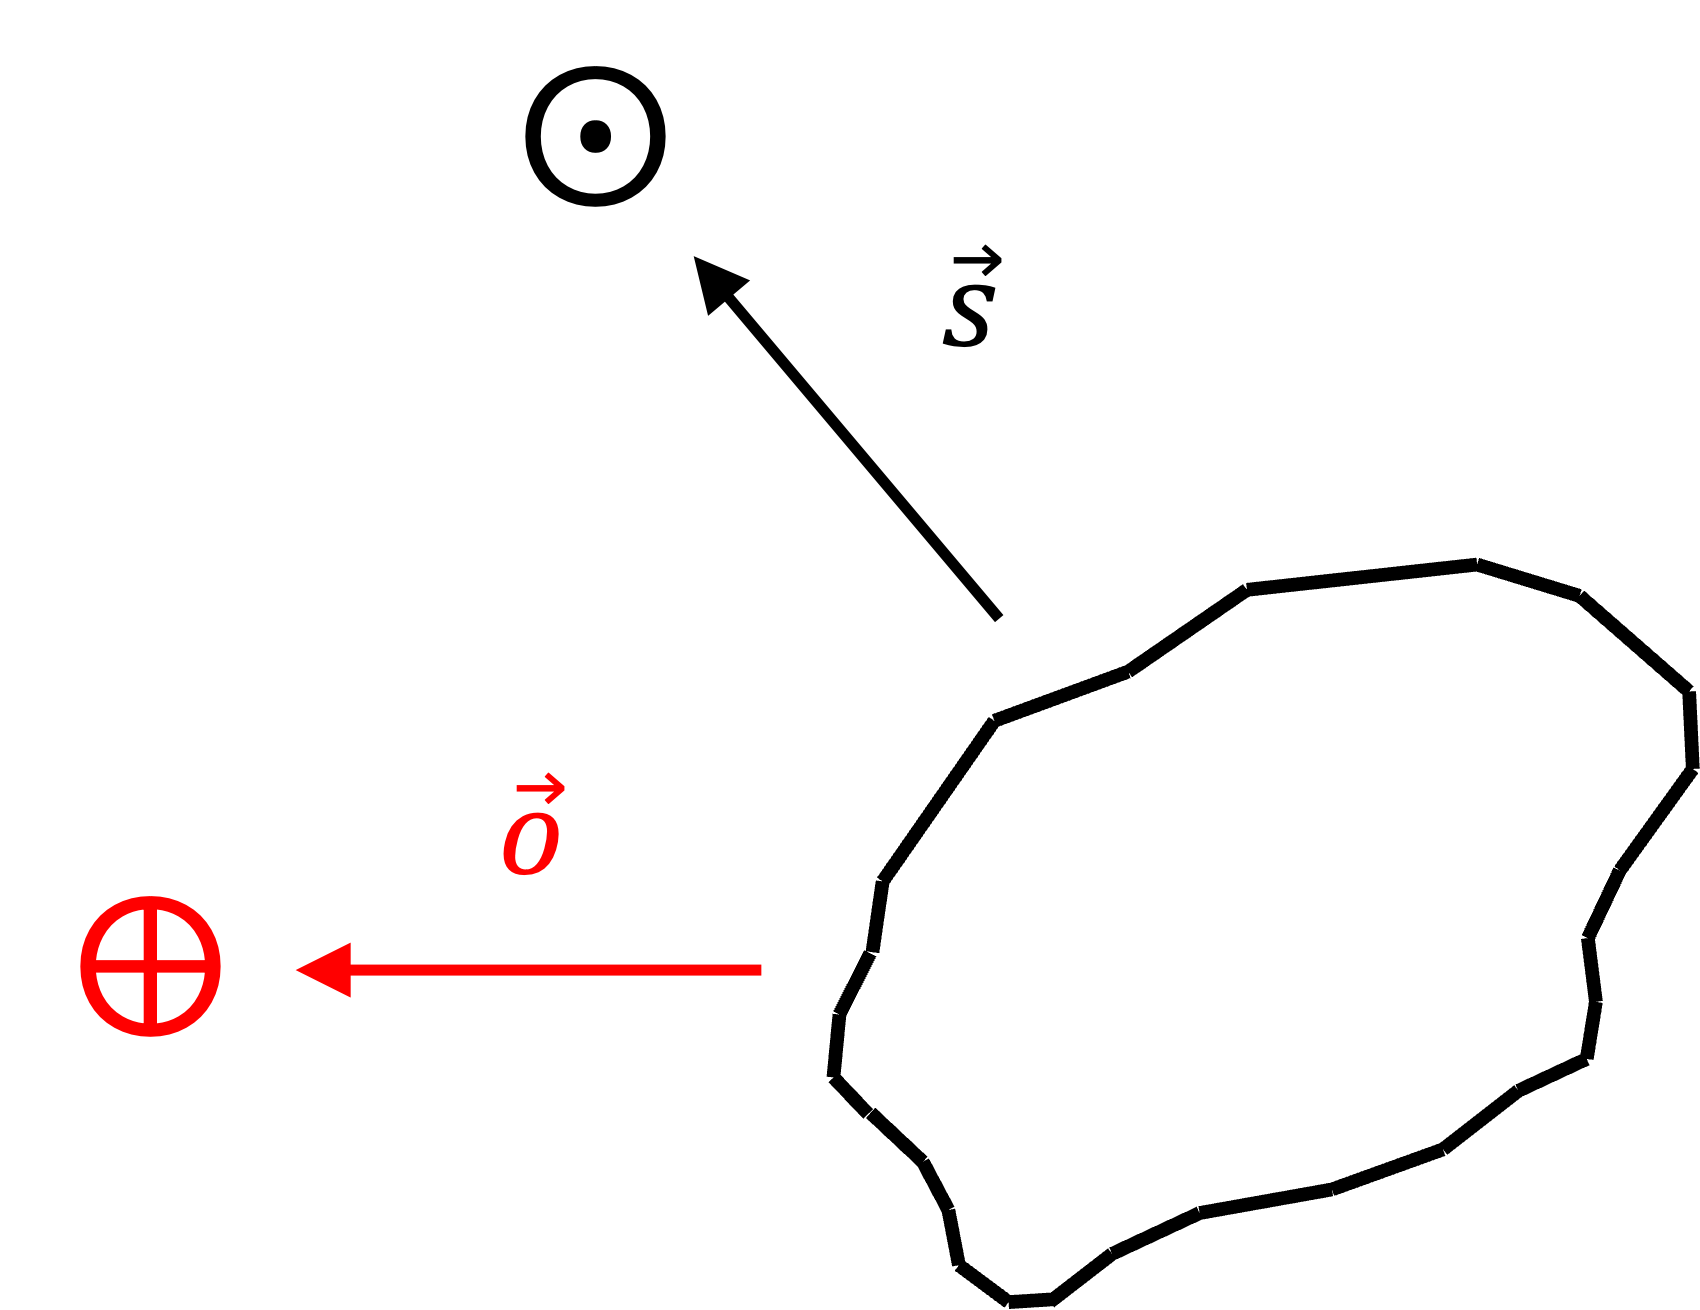
\includegraphics[scale=0.425]{figs/schema.png}
\centering
\caption{Ukázka vektorů $\vec s$ (směru ke Slunci) a $\vec o$ (směru k pozorovateli) vůči asteroidu.}
\label{schema}
\end{figure}

Ze světelných křivek byly odvozeny desetitisíce modelů asteroidů \cite{Durech_2023A&A...675A..24D,Broz_2023A&A...676A..60B}. Nástroje pro jejich vizualizaci sice existují, ale stávající programy jsou dosti jednoduché a pomalé. Cílem mojí práce je vytvořit jednotný program, který asteroidy efektivně vizualizuje a kreslí jejich světelné křivky, za použití moderního programovacího jazyka a akcelerované grafické knihovny. 

\iffalse
rozvest damit, neni jen pro me - vyznam pro ostatni
\fi

%%%%%%%%%%%%%%%%%%%%%%%%%%%%%%%%%%%%%%%%%%%%%%%%%%%%%%%%%%%%%%%%%%%%%%

\newpage
\section{Teoretické koncepty programu}

Teoretická část popisuje koncepty důležité pro hlubší pochopení programu. Všechny z nich jsou jeho nedílnou součástí a jeho fungování na nich závisí. 

\subsection{Asteroidy}

Asteroidy jsou vesmírná tělesa, velká jednotky metrů až stovky kilometrů. Ty největší se od Země nachází typicky 1,5 astronomických jednotek daleko (1\,au = 149,6 milionů kilometrů) a na obloze zabírají řádově jednu desetinu úhlové vteřiny ($100\,{\rm km} / 1,5\,{\rm au} = 4.5\cdot 10^{-7}\,{\rm rad} = 0.1''$). Pouhým okem tak není poznat že se jedná o asteroid. Jejich viditelnost ještě zhoršuje chvění vzduchu, které rozmazává obraz o zhruba jednu úhlovou vteřinu. Chvění vzduchu je jev způsobený zemskou atmosférou, ve které vrstvy vzduchu fungují jako malé čočky, lomící světelné paprsky. 

\begin{figure}[h]
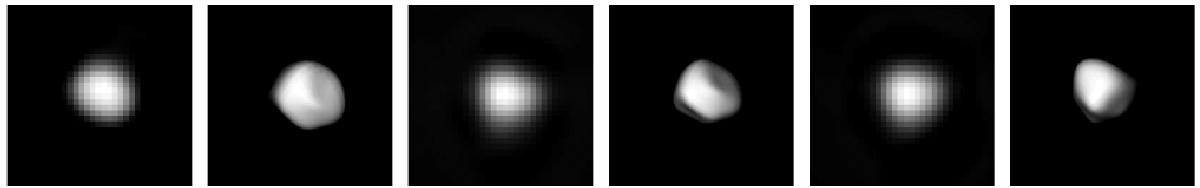
\includegraphics[width=15cm]{figs/adaptive_optics_asteroids.png}
\centering
\caption{Obrázky asteroidu 354 Eleonora z adaptivní optiky a jeho modely.
Převzato z~\cite{Viikinkoski_2017A&A...607A.117V}.}
\label{adaptive_optics_asteroids}
\end{figure}

Při pozorování asteroidů tedy musíme spoléhat na jiné přístroje než naše oči. Adaptivní optika dokáže korigovat chvění vzduchu a zvětšit vesmír před objektivem natolik, že jsou asteroidy rozpoznatelné (obr.~\ref{adaptive_optics_asteroids}). Pro pozorování těch malých ale ani adaptivní optika nestačí, a tak se astronomové musí spoléhat na jiné metody. Nejdetailnějšího popisu tvaru se dosáhne vysláním sondy přímo k asteroidu, která ho snímkuje z oběžné dráhy, a zaznamená tak i topografii povrchu.


%%%%%%%%%%%%%%%%%%%%%%%%%%%%%%%%%%%%%%%%%%%%%%%%%%%%%%%%%%%%%%%%%%%%%%

\subsection{Triangulace tvaru}

Tvar asteroidů není možné zachytit dokonale přesně. Asteroidy jsou totiž tvarem nepravidelné, některé části mají oblé, jiné rovné, hladké, drsné --- takový tvar je počítačem velmi těžké popsat. Svoji práci si usnadňujeme tím, že tvar popisujeme jen {\em zhruba\/}, a to rozdělením povrchu tělesa na menší a jednodušší části. Jednou částí může být trojúhelník, který je svým tvarem jednoduchý --- lze pro něj například snadno vyčíslit obsah. 

\begin{figure}[h!]
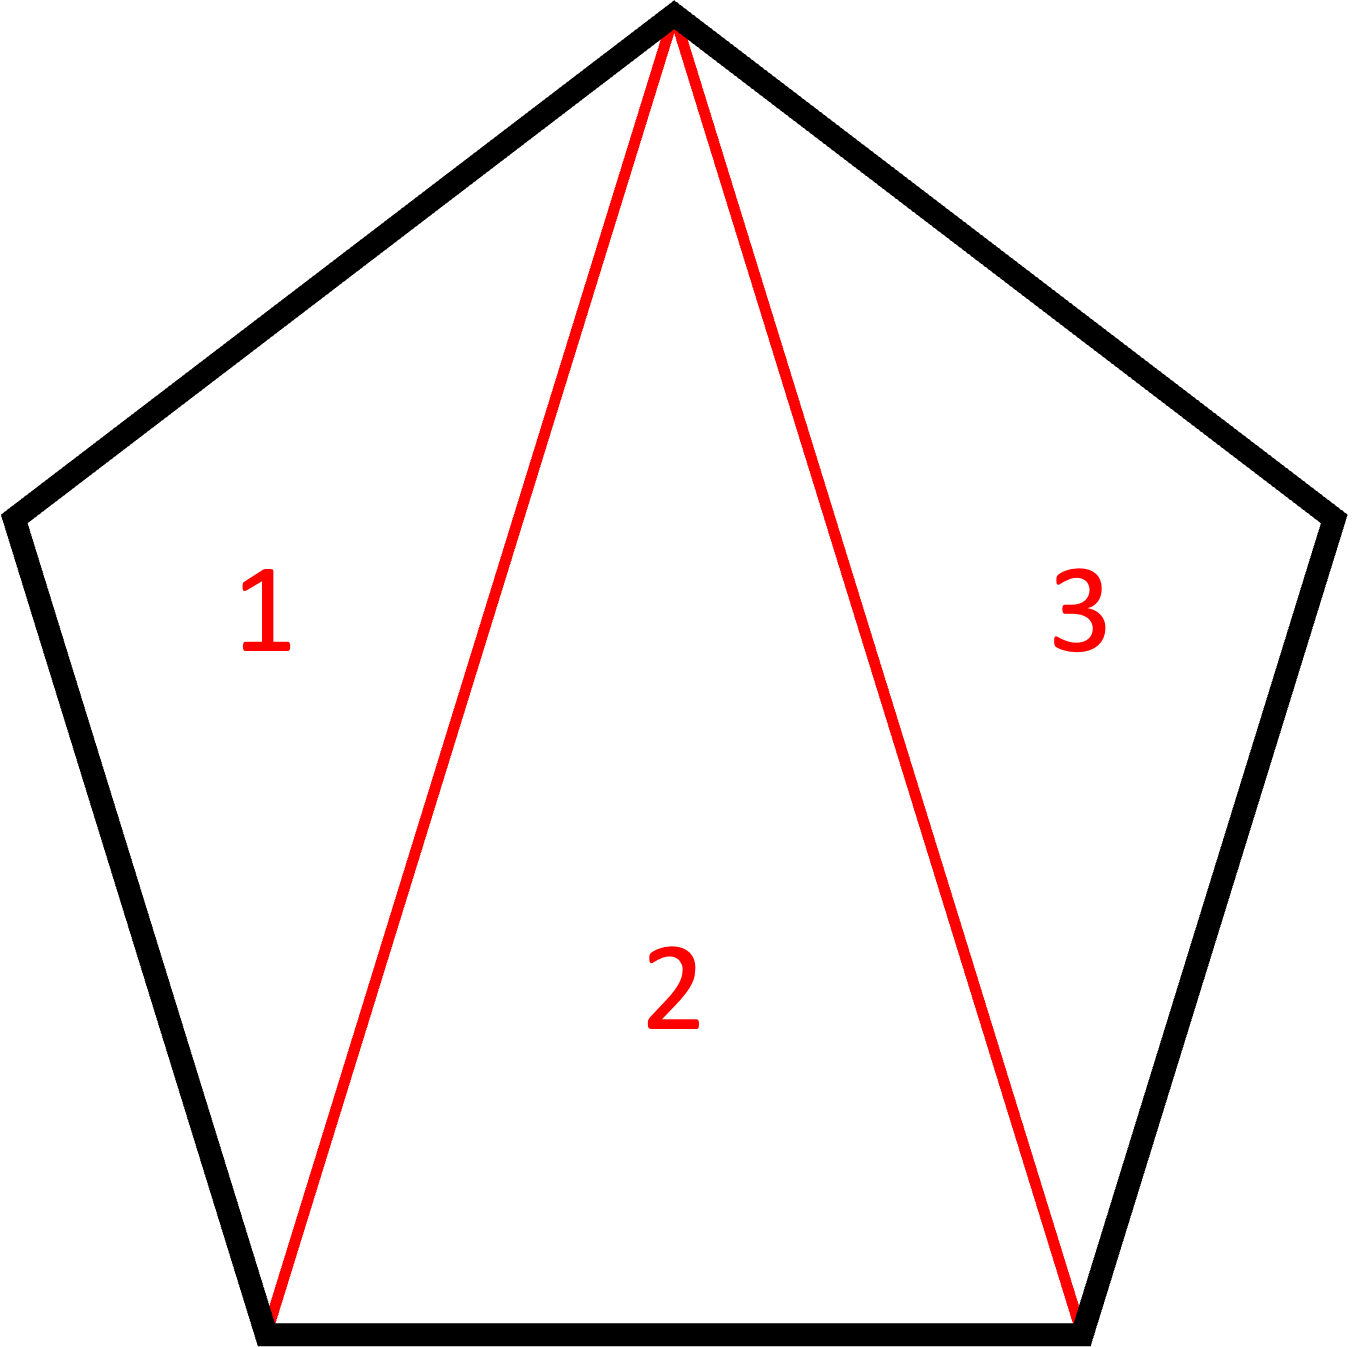
\includegraphics[scale=0.3]{figs/triangulation.png}
\centering
\caption{Ukázka triangulace pětiúhelníku.}
\label{triangulation}
\end{figure}

Procesu rozdělení povrchu na trojúhelníkové plošky se říká triangulace. S~triangulací se můžeme setkat například při výpočtu obsahů složitějších útvarů. Ty se často dělí právě na soubor trojúhelníku, u kterých obsah spočítat umíme (obr.~\ref{triangulation}). 

Trojrozměrný tvar asteroidu se v databázích ukládá jako soubor kartézských souřadnic vrcholů trojúhelníků a indexů, které určují, jaké tři vrcholy tvoří jeden trojúhelník. Jednou takovou databází je DAMIT \cite{Durech_2023A&A...675A..24D}. Formát se nazývá \verb|.obj| a je pro modelování tvarů asteroidů tím nejrozšířenějším.

%%%%%%%%%%%%%%%%%%%%%%%%%%%%%%%%%%%%%%%%%%%%%%%%%%%%%%%%%%%%%%%%%%%%%%

\subsection{Vlastnosti trojúhelníku}

Trojúhelníky v prostoru mají unikátní soubor vlastností. Všechny pro nás důležité vlastnosti jsou shrnuté v následujícím seznamu~\cite{Rektorys_2009}.
Obvod je:
\begin{equation}
o = a + b + c\,,
\end{equation}
kde $a$, $b$, $c$ označují délky stran.

Délka strany:
\begin{equation}
a = |\vec B - \vec C|\,,
\end{equation}
kde $\vec A$, $\vec B$, $\vec C$ označují vektory z~počátku souřadné soustavy~$\vec O$ do příslušného vrcholu.
Ostatní strany je možné spočítat cyklickou záměnou.

Součet úhlů:
\begin{equation}
\alpha + \beta + \gamma = 180^\circ\,.
\end{equation}

Obsah:
\begin{equation}
S = {a V_a\over 2}\,,
\end{equation}
kde $v_a$ je výška příslušná straně $a$.
Alternativně:
\begin{equation}
S = {1\over 2}|(\vec B-\vec C) \times (\vec C-\vec A)|\,,
\end{equation}
kde operace vektorového součinu ($\times$) je definována jako:
\begin{equation}
\vec a\times\vec b = (a_2 b_3 - a_3 b_2; a_3 b_1 - a_1 b_3; a_1 b_2 - a_2 b_1)\,.
\end{equation}

Těžiště:
\begin{equation}
\vec T = {1\over 3}(\vec A + \vec B + \vec C)\,.
\end{equation}

Sevřený úhel:
\begin{equation}
\cos\gamma = {(\vec B-\vec C)\cdot (\vec A-\vec C)\over |\vec B-\vec C| |\vec A-\vec C|}\,,
\end{equation}
kde operace skalárního součinu ($\cdot$) je definována následovně:
\begin{equation}
\vec a \cdot \vec b = a_1 b_1 + a_2 b_2 + a_3 b_3\,.
\end{equation}
Ostatní úhly je možné spočítat cyklickou záměnou.

Normála:
\begin{equation}
\vec n = {(\vec B-\vec C) \times (\vec C-\vec A)\over |(\vec B-\vec C) \times (\vec C-\vec A)|}\,,
\end{equation}
kde jmenovatel zajišťuje normalizaci na délku 1.

První směrový kosinus:
\begin{equation}
\mu_{\rm i} = \vec s\cdot \vec n\,,
\end{equation}
kde $\vec s$ je vektor mířící ke Slunci.

Druhý směrový kosinus:
\begin{equation}
\mu_{\rm e} = \vec o\cdot \vec n\,,
\end{equation}
kde $\vec o$ je vektor mířící k pozorovateli.
Promítnutá plocha:
\begin{equation}
S' = \mu_{\rm e} S\,,
\end{equation}
kde $S'$ je pro pozorovatele viditelná plocha.

Posunutí o vektor $\vec O'$:
\begin{eqnarray}
\vec A' &=& \vec A + \vec O'\,,\\ 
\vec B' &=& \vec B + \vec O'\,,\\ 
\vec C' &=& \vec C + \vec O'\,.
\end{eqnarray}
Posunutí trojúhelníku o vektor $\vec O'$ spočívá v posunutí všech jeho vrcholů.

Otočení okolo osy $z$ o~úhel~$\phi$:
\begin{eqnarray}
A_1' &=& A_1\cos\phi - A_2\sin\phi\,,\\
A_2' &=& A_1\sin\phi + A_2\cos\phi\,,\\
A_3' &=& A_3\,.
\end{eqnarray}
Ostatní vrcholy obdobně.
Ostatní otočení také obdobně.

%  A
%  |\
%  | \ 
%  |  \
%  -----
%  B   C
 
%%%%%%%%%%%%%%%%%%%%%%%%%%%%%%%%%%%%%%%%%%%%%%%%%%%%%%%%%%%%%%%%%%%%%%

\subsection{Rozptyl světla}

V síti trojúhelníků má každý svoji vlastní míru osvětlení. Osvětlení je způsobené tokem světelného záření od Slunce (označovaný $\Phi_\odot$). Hodnota toku se udává ve ${\rm W}\,{\rm m}^{-2}$ a ve vzdálenosti Země dosahuje hodnoty $1361\,{\rm W}\,{\rm m}^{-2}$. Pro odlišné vzdálenosti se počítá jako:
\begin{equation}
\Phi = {P\over 4\pi r^2}\,,
\end{equation}
kde $P$ označuje zářivý výkon Slunce ($3,827 \cdot 10^{26}\,{\rm W}$) a $r$ vzdálenost od Slunce.

To, jak trojúhelník je (či není) osvětlený závisí na úhlu, pod jakým paprsky světla dopadají. Rovnici pro výpočet toku na trojúhelník musíme upravit tak, aby tento úhel brala v potaz \citep{Broz_2013}:
\begin{equation}
\Phi_{\rm i} = \Phi \mu_{\rm i}\,,
\end{equation}
kde $\mu_{\rm i}$ je první směrový kosinus. Je-li první směrový kosinus záporný, rovná se $\Phi_{\rm i}$ nule (trojúhelník je odkloněný). U extrémních úhlů může dojít ke stínění, které je způsobené nerovnostmi na povrchu. Jedná-li se o konvexní povrch, ke stínění nedochází.  

Povrch asteroidu rozptyluje světelné paprsky do různých směrů --- je vidět i pod úhlem různým od úhlu dopadu (obr.~\ref{dispersion}). Tento rozptyl je způsoben mikroskopickými nerovnostmi, od kterých se paprsky odrážejí. Intenzita $I$ rozptýleného záření se obecně počítá jako:
\begin{equation}
I = f \Phi_{\rm i}\,,
\end{equation}
kde $f$ je funkce rozptylu, která popisuje souvislost mezi dopadajícími a rozptýlenými paprsky. Funkcí rozptylu existuje celá řada. Vzájemně se mezi sebou liší složitostí a přesností popisu rozptylu. Nejjednodušší je Lambertova funkce rozptylu:
\begin{equation}
f = f_{\rm L}\,,
\end{equation}
kde $f_{\rm L}$ je konstanta, která charakterizuje materiál povrchu. Další, komplexnější funkcí je Lommelova--Seeligerova funkce rozptylu: 
\begin{equation}
f = {f_{\rm L}\over\mu_{\rm i}+\mu_{\rm e}}
\end{equation}
kde se konstanta dodatečně dělí součtem prvního a druhého směrového kosinu --- tato funkce lépe popisuje preferovaný rozptyl paprsků do stran. Ještě přesněji by rozptyl popisovala Hapkeho funkce \citep{Hapke_1984Icar...59...41H,Spjuth_2009PhDT.......588S}.

Tok rozptýleného záření z trojúhelníku je potom:
\begin{equation}
\Phi_{\rm e} = I \mu_{\rm e}\,,
\end{equation}
kde $\mu_{\rm e}$ je druhý směrový kosinus.

\begin{figure}[h!]
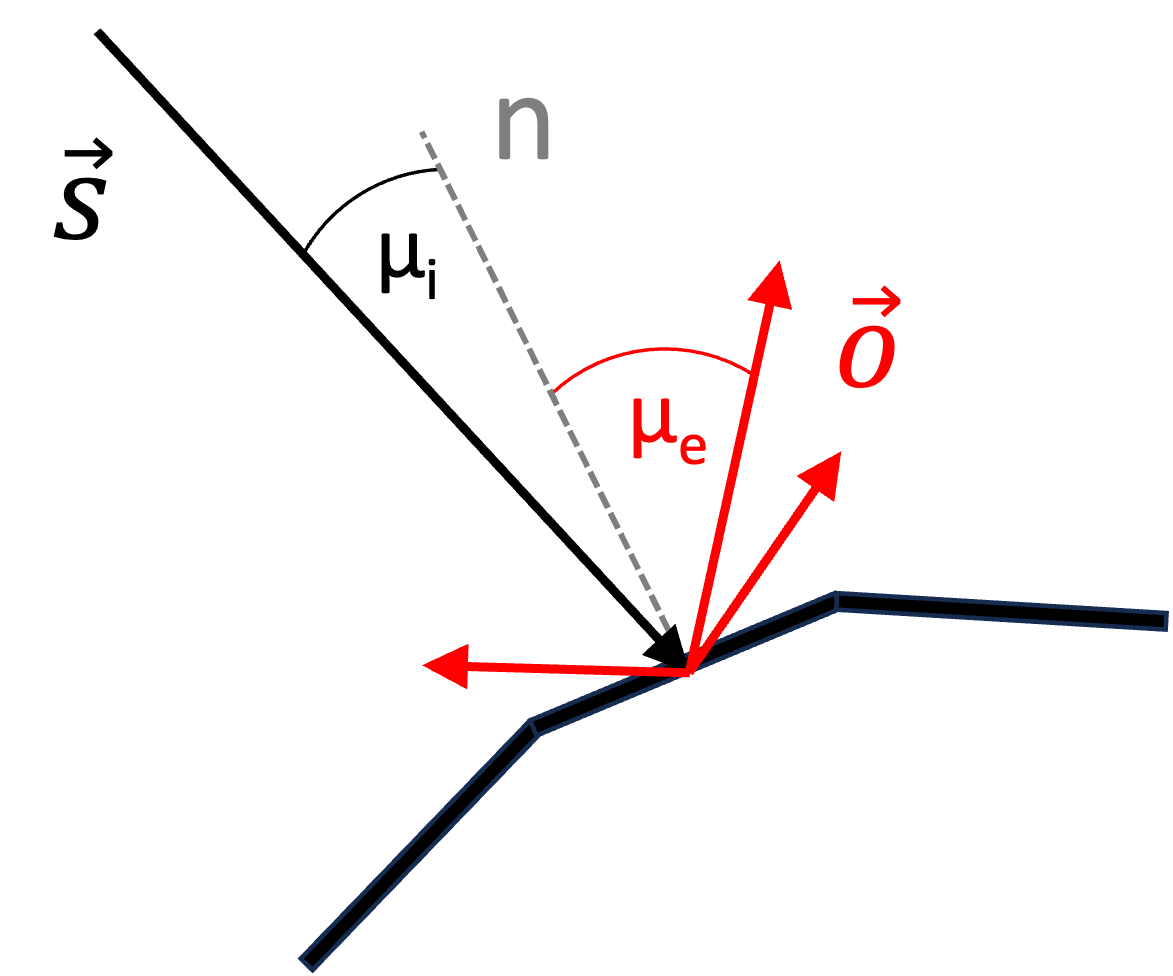
\includegraphics[scale=0.425]{figs/dispersion.png}
\centering
\caption{Ilustrace rozptylu světla po dopadu na povrch asteroidu.}
\label{dispersion}
\end{figure}


%%%%%%%%%%%%%%%%%%%%%%%%%%%%%%%%%%%%%%%%%%%%%%%%%%%%%%%%%%%%%%%%%%%%%%

\subsection{Světelná křivka}

Když se po určitou dobu pozorují paprsky rozptýlené asteroidem, vznikne světelná křivka. Světelná křivka je tedy součtem toků přicházejících od jednotlivých trojúhelníků; matematicky vyjádřeno:
\begin{equation}
\Phi = \int \Phi_{\rm e}(\vec r) {\rm d} S = \sum_j \Phi_{\rm e}(j) {\rm d} S_j\,,
\end{equation}
kde trojúhelníky indexujeme písmenem $j$.

Otáčení asteroidu způsobuje na světelné křivce výkyvy (obr.~\ref{22_test48_update2_output.0001.syn}, \ref{22_test48_update2_chi2_LC2_PHASE}). Ty jsou znakem změn v~odrazové ploše asteroidu. Společně s odrazovou plochou se mění i~toky rozptýleného záření od jednotlivých trojúhelníků. Součet jejich hodnot je zaznamenaný v~grafu světelné křivky na ose $y$; na ose $x$ je čas. Z grafu světelné křivky tak lze odvodit periodu otáčení asteroidu i~jeho přibližný tvar. 

% Tohle je trochu matoucí. Celkový tok je dán integrálem přes povrch, v naší reprezentaci sumou přes trojúhelníky. Protože se geometrie mění s časem, mění se i tok. Nejrychlejší a periodickou změnou je změna díky rotaci planetky, tomu se říká světelná křivka.}

\begin{figure}[p]
\centering
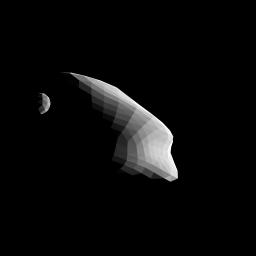
\includegraphics[width=3.5cm]{figs/22_test48_update2/output.0001.syn.png}
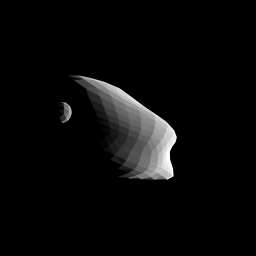
\includegraphics[width=3.5cm]{figs/22_test48_update2/output.0002.syn.png}

\includegraphics[width=3.5cm]{figs/22_test48_update2/output.0003.syn.png}

\includegraphics[width=3.5cm]{figs/22_test48_update2/output.0004.syn.png}

\includegraphics[width=3.5cm]{figs/22_test48_update2/output.0005.syn.png}

\includegraphics[width=3.5cm]{figs/22_test48_update2/output.0006.syn.png}
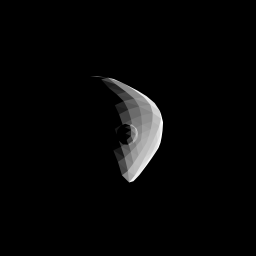
\includegraphics[width=3.5cm]{figs/22_test48_update2/output.0007.syn.png}

\includegraphics[width=3.5cm]{figs/22_test48_update2/output.0008.syn.png}
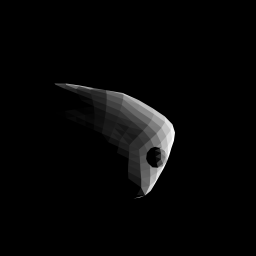
\includegraphics[width=3.5cm]{figs/22_test48_update2/output.0009.syn.png}

\includegraphics[width=3.5cm]{figs/22_test48_update2/output.0010.syn.png}

\includegraphics[width=3.5cm]{figs/22_test48_update2/output.0011.syn.png}
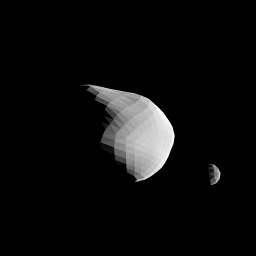
\includegraphics[width=3.5cm]{figs/22_test48_update2/output.0012.syn.png}
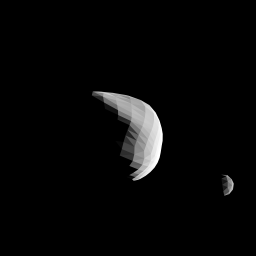
\includegraphics[width=3.5cm]{figs/22_test48_update2/output.0013.syn.png}
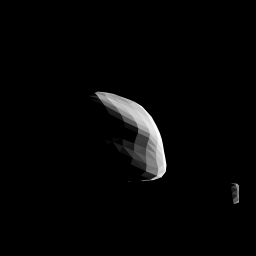
\includegraphics[width=3.5cm]{figs/22_test48_update2/output.0014.syn.png}
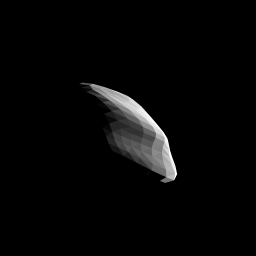
\includegraphics[width=3.5cm]{figs/22_test48_update2/output.0015.syn.png}

\includegraphics[width=3.5cm]{figs/22_test48_update2/output.0016.syn.png}
%\vskip.3cm
%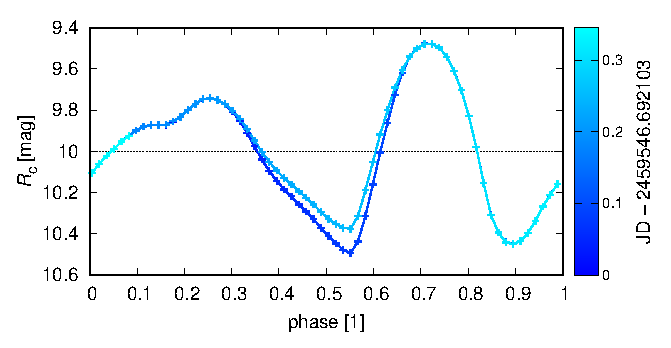
\includegraphics[width=10cm]{figs/22_test48_update2/chi2_LC2_PHASE.eps}
\caption{
Model asteroidu (22) Kalliope a~jeho měsíce Linus.
Převzato z~\cite{Broz_2023A&A...676A..60B}.
}
\label{22_test48_update2_output.0001.syn}
\end{figure}


\begin{figure}
\centering
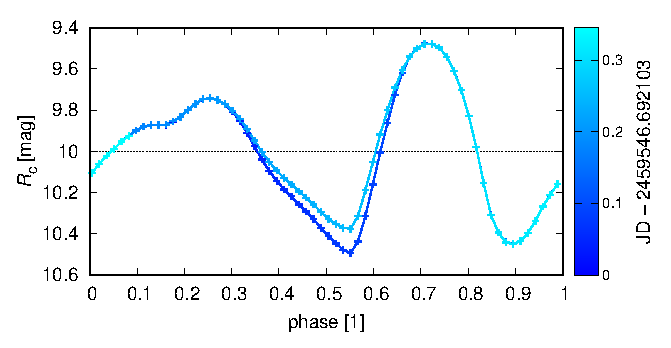
\includegraphics[width=10cm]{figs/22_test48_update2/chi2_LC2_PHASE.eps}
\caption{
Světelná křivka odpovídající obr.~\ref{22_test48_update2_output.0001.syn}.}
\label{22_test48_update2_chi2_LC2_PHASE}
\end{figure}



%%%%%%%%%%%%%%%%%%%%%%%%%%%%%%%%%%%%%%%%%%%%%%%%%%%%%%%%%%%%%%%%%%%%%%

\newpage
\clearpage
\section{Technické řešení programu}

Technické řešení popisuje zdrojový kód programu, použité nástroje a postup vývoje. Program je strukturovaný do čtyř souborů. Hlavního (\verb|Main.py|), kde je uložená většina kódu aplikace, a~tří vedlejších, podpůrných. \verb|Load.py| se stará o načtení a zpracování \verb|.obj| souboru, \verb|Shadowing.py| počítá zákryt trojúhelníků a \verb|Hapke.py| počítá složitou Hapkeho funkci rozptylu. 

%progamovaci jazyk python - interpretovany, objektovy, proc on, zminit sbpy \cite{Mommert_2019JOSS....4.1426M} a vispy \cite{vispy} interaktivni akcelerovana knihovna, jeji vyznam v projektu

\subsection{Nástroje}

Celá aplikace je napsaná v programovacím jazyce Python3 \cite{python}.
Python je interpretovaný a~objektově orientovaný jazyk, je v něm tedy lehké napsat přehledný a stručný program.
Mimo jiného má vzhledem k jeho popularitě nejširší nabídku knihoven, na kterých lze aplikace podobné té mojí stavět. 

Aplikace je založena na knihovně VisPy \cite{vispy}, která se po vyzkoušení jiných jevila jako nejlepší. Jedná se o~multiplatformní akcelerovanou knihovnu pro vizualizaci. Poskytuje přístup k funkcím výkonných grafických karet, a to pomocí připravených vysokoúrovňových objektů a metod.


%%%%%%%%%%%%%%%%%%%%%%%%%%%%%%%%%%%%%%%%%%%%%%%%%%%%%%%%%%%%%%%%%%%%%%

\subsection{Načítání souboru .obj}

Jedním z prvních úkolů při vývoji je načítání souboru \verb|.obj|. Ten slouží jako vstupní formát dat pro celou aplikaci. Soubor \verb|.obj| obsahuje vrcholy a stěny 3D modelu. Řádky s vrcholy začínají písmenem v a skládají se ze tří dalších čísel; $x$, $y$, $z$ souřadnic vrcholu. Ten samý soubor také obsahuje řádky začínající písmenem f. Následující čísla určují, jaké tři vrcholy tvoří jeden trojúhelník.

\lstinputlisting[language=Python]{python_scripts/3_2/obj_sample.py}

Naším cílem je vytvořit jednoduchou funkci, která rozdělí data na listy samotných vrcholů a~samotných stěn. Funkce bere jako argument cestu k souboru, zbaví data písmen na začátku řádků a rozliší řádky s vrcholy a stěnami.
Využívá se systémové funkce \verb|map()|, která zavolá určitou funkci pro každý prvek listu.
Přitom je možné použít operátor \verb|lambda|, který určitou proměnnou nahradí za výraz.

\lstinputlisting[language=Python]{python_scripts/3_2/load_function.py}

% kde se berou .obj - svetelna krivka -> .obj,

%%%%%%%%%%%%%%%%%%%%%%%%%%%%%%%%%%%%%%%%%%%%%%%%%%%%%%%%%%%%%%%%%%%%%%

\subsection{Třída Asteroid()}

Než definujeme třídu asteroidu, musíme importovat všechny knihovny, které bude program používat. Až do čtrnáctého řádku jde o knihovny volně dostupné na internetu. Další tři jsou mnou naprogramované knihovny. Knihovna \verb|Shadowing.py| je kvůli rychlosti naprogramovaná v jazyce Fortran 90. Aby mohl Python Fortranovský soubor přečíst, používá knihovnu fmodpy.

\lstinputlisting[language=Python]{python_scripts/3_4/imports.py}

Na začátku programu také definujeme funkce pro výpočet rozptylu světla. Lambertův anebo Lommelův--Seeligerův rozptyl je natolik jednoduchý, že se vejde na pár řádků. Funkce pro Hapkeho rozptyl \cite{Hapke_1984Icar...59...41H,Spjuth_2009PhDT.......588S} má kolem sto padesáti řádků, je proto umístěna v separátním souboru. 

\lstinputlisting[language=Python,firstnumber=last]{python_scripts/3_4/dispersion_functions.py}

Třída \verb|Asteroid| začíná konstruktorem, který bere jako parametry terminálové argumenty a~cestu k~souboru. Následně jsou definované proměnné instance třídy, čili objektu (\verb|self.|). Program načítá data asteroidu knihovnou \verb|Load|, konkrétně její funkcí \verb|load_obj()|. 

\lstinputlisting[language=Python,firstnumber=last]{python_scripts/3_4/asteroid_class.py}

%%%%%%%%%%%%%%%%%%%%%%%%%%%%%%%%%%%%%%%%%%%%%%%%%%%%%%%%%%%%%%%%%%%%%%

\subsection{Výpočet fyzikálních vlastností}

Aby byl model asteroidu realistický, musí být založený na reálných výpočtech. Příslušná metoda \verb|get_geometry()| počítá těžiště a normály trojúhelníků. 

\lstinputlisting[language=Python,firstnumber=last]{python_scripts/3_5/get_geometry_head.py}

V každém cyklu metoda uloží vrcholy trojúhelníku do proměnných \verb|A|, \verb|B| a \verb|C|. Spočítaná těžiště a~normály se poté ukládají do předem definovaných listů.

\lstinputlisting[language=Python,firstnumber=last]{python_scripts/3_5/get_geometry.py}

Metoda \verb|get_cosines()| počítá směrové kosiny trojúhelníků a jejich stínění. Jako argumenty bere vektory $\vec s$~(směr, ze kterého svítí Slunce) a $\vec o$ (směr, ze kterého se dívá pozorovatel). 

\lstinputlisting[language=Python,firstnumber=last]{python_scripts/3_5/get_cosines_head.py}

První a druhý směrový cosinus každého trojúhelníku se ukládá ve \verb|for| cyklu do listů, respektive numpyovských polí. Z polí jsou pak vyřazeny záporné hodnoty směrových kosinů; jedná se totiž o trojúhelníky, které se nacházejí na odvrácené straně asteroidu, nebo nesměřují ke Slunci/pozorovateli. 

\lstinputlisting[language=Python,firstnumber=last]{python_scripts/3_5/get_cosines.py}

Pro výpočet příchozích (\verb|phi_i|) a rozptýlených (\verb|phi_e|) světelných toků používá program metodu \verb|get_fluxes()|. Příchozí tok na trojúhelník se spočítá jako násobek toku od slunce (\verb|phi_s|), prvního směrového kosinu a veličiny \verb|nu_i|, která se v případě, že je trojúhelník zastíněný jiným trojúhelníkem, rovná nule, jinak jedné. Před výpočtem rozptýleného (odraženého) toku metoda nejprve provede \verb|for| cyklus, kde do listu uloží hodnoty dle vybrané funkce rozptylu.   

\lstinputlisting[language=Python,firstnumber=last]{python_scripts/3_5/get_fluxes.py}

Na konci metoda provede sumu rozptýlených toků. Ta se použije k~výpočtu světelné křivky. 

%%%%%%%%%%%%%%%%%%%%%%%%%%%%%%%%%%%%%%%%%%%%%%%%%%%%%%%%%%%%%%%%%%%%%%

\subsection{Výpočet světelné křivky}

Ještě než program přejde k vizualizaci, spočítá světelnou křivku. Jako argument bere metoda \verb|light_curve()| počet kroků, které na jedno otočení kolem osy udělá. U každého úhlu spočítá metoda celkový rozptýlený tok a uloží ho do listu \verb|total|.

\lstinputlisting[language=Python,firstnumber=last]{python_scripts/3_6/light_curve.py}

List je pak převeden na numpyovské pole a uložen do textového souboru s názvem \verb|light_curve.txt|. Aby se světelná křivka dala dobře vykreslit na obrazovku, musejí se její hodnoty normalizovat. Normalizované hodnoty se pak předají třídě \verb|Line()| knihovny VisPy, která je vykreslí na obrazovku v podobě světelné křivky.

\lstinputlisting[language=Python,firstnumber=last]{python_scripts/3_6/light_curve_end.py}

%%%%%%%%%%%%%%%%%%%%%%%%%%%%%%%%%%%%%%%%%%%%%%%%%%%%%%%%%%%%%%%%%%%%%%

\subsection{Vizualizace pomocí knihovny VisPy}

\subsubsection{Příklad trojúhelníku}

Pro lepší pochopení toho, jak knihovna VisPy funguje, načteme nejdříve samotný trojúhelník a~spočítáme jeho normálu. Abychom mohli knihovnu používat, musíme ji nejdříve do programu importovat. K~práci se nám také bude hodit knihovna NumPy \cite{numpy}.

\lstinputlisting[language=Python]{python_scripts/3_7/3_7_1/imports.py}

Začneme definováním funkce \verb|main()|, která je volaná po spuštění programu. V ní zavedeme proměnou \verb|canvas|, která reprezentuje okno aplikace, a nastavíme jeho velikost.   

\lstinputlisting[language=Python,firstnumber=last]{python_scripts/3_7/3_7_1/define_function.py}

Vrcholy trojúhelníku ABC jsou definovány třírozměrnými souřadnicemi. Ty jsou zároveň obaleny funkcí \verb|np.array()|, která převádí datový typ list na pole pro rychlé výpočty.

\lstinputlisting[language=Python,firstnumber=last]{python_scripts/3_7/3_7_1/vertices.py}

Pro zobrazení normály trojúhelníku potřebujeme znát jeho těžiště. Těžiště se nachází v průsečíku těžnic. Ty jsou spojnicí vrcholu a středu protější strany. Střed strany $a$ se spočítá jako absolutní hodnota rozdílu vektorů $\vec B$ a $\vec C$. Ostatní středy se spočítají obdobně, jak lze vidět níže.

\lstinputlisting[language=Python,firstnumber=last]{python_scripts/3_7/3_7_1/calculations.py}

Všechny dosavadní kroky se odehrávaly pouze v paměti programu. Definované věci musíme ještě vykreslit na obrazovku. Vykreslování jednotlivých objektů je vidět v následujícím úryvku kódu:

\lstinputlisting[language=Python,firstnumber=last]{python_scripts/3_7/3_7_1/visuals.py}

Nakonec se zvolí poloha kamery,
přidají souřadnicové osy $x$, $y$, $z$,
zobrazí připravený canvas
a~pomocí \verb|vispy.app.run()| se předá řízení smyčce knihovny.

\lstinputlisting[language=Python,firstnumber=last]{python_scripts/3_7/3_7_1/end.py}

Produktem popsaného programu je trojúhelník na obrázku~\ref{triangle_example}.
Je možné jej interaktivně ovládat.

\begin{figure}[h]
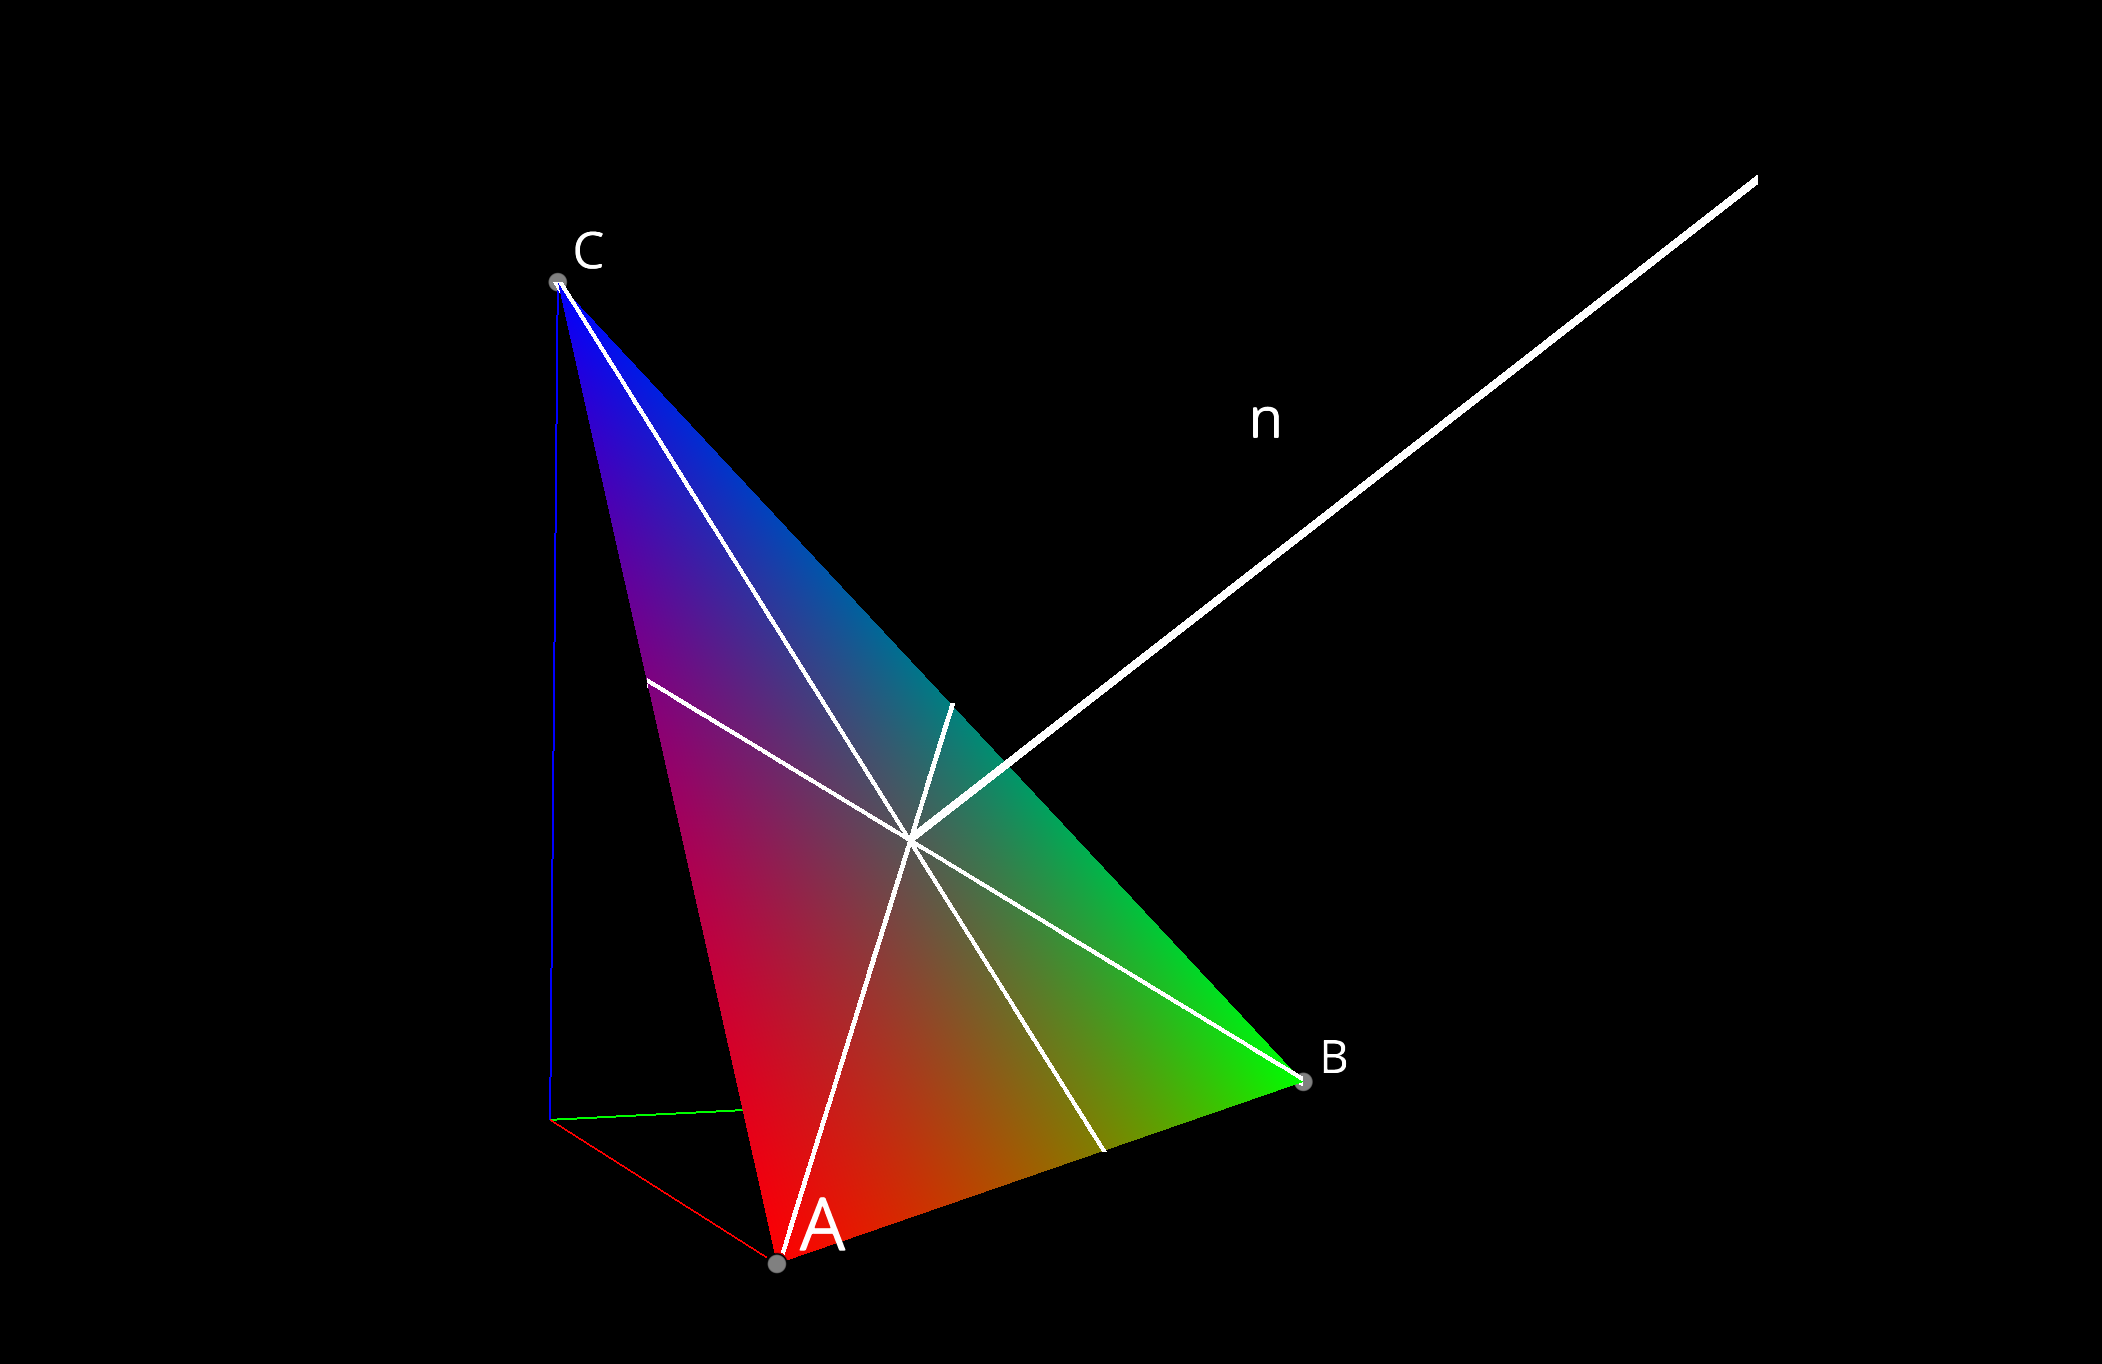
\includegraphics[width=10cm]{figs/triangle_example.png}
\centering
\caption{Ukázka trojúhelníku zobrazeného knihovnou VisPy.}
\label{triangle_example}
\end{figure}

%%%%%%%%%%%%%%%%%%%%%%%%%%%%%%%%%%%%%%%%%%%%%%%%%%%%%%%%%%%%%%%%%%%%%%

%\newpage
\subsubsection{Příklad asteroidu}

Knihovna VisPy zobrazuje model celého asteroidu obdobně jako trojúhelník samotný. Na začátku metody \verb|plot()| definujeme okno programu, jeho velikost a obraz v něm.

\lstinputlisting[language=Python,firstnumber=114]{python_scripts/3_7/3_7_2/plot_head.py}

Knihovna VisPy má pro síť spojených bodů zavedenou třídu \verb|Mesh()|, která bere jako argumenty listy vrcholů, stěn a barev plošek. Nastavení parametru \verb|color=| aplikuje vybranou barvu na všechny plošky.

\lstinputlisting[language=Python,firstnumber=last]{python_scripts/3_7/3_7_2/mesh.py}

Metoda poté přejde k vizualizaci už spočítaných normál. Ty jsou vykreslené třídou \verb|Line()|, které se předají souřadnice začátků a konců normál a informace o tom, který začátek a konec patří k sobě. List s těmito informacemi neumí knihovna VisPy vytvořit sama, je tak vytvořený jednoduchým \verb|for| cyklem. Viditelnost normál je jako výchozí nastavená na \verb|False|; v základním zobrazení nejsou vidět.

\lstinputlisting[language=Python,firstnumber=last]{python_scripts/3_7/3_7_2/normals.py}

V kódu jsou používané dva různé způsoby přidávaní objektů na obrazovku, metoda \verb|self.view.add()| a~argument \verb|parent=self.view.scene|. V~tom, jak se objekty zobrazí\jd{,} rozdíl není. Způsob s~\verb|self.view.add()| se používá, když se jedná o objekt, který se dále upravuje (např. objekt \verb|normals|, kterému se upravuje viditelnost). Aby byl program přehledný, vykreslují se na obrazovku vysvětlivky v~podobě textu a~významných vektorů. 

\lstinputlisting[language=Python,firstnumber=last]{python_scripts/3_7/3_7_2/info.py}

Knihovna VisPy používá třídu \verb|ShadingFilter()| pro vykreslování asteroidu Phongovou metodou (standardní metoda na vykreslování a nasvícení 3D objektu, která nepočítá stínění) a třídu \verb|WireframeFilter| pro dodatečné vykreslování sítě.

\lstinputlisting[language=Python,firstnumber=182]{python_scripts/3_7/3_7_2/filters.py}

Funkce \verb|plot_fluxes()| slouží jako zestručnění kódu, který by se jinak u~ovládání klávesami mnohokrát opakoval. Funkce bere jako argument veličinu (\verb|phi|) a vykresluje hrubý model asteroidu s~viditelnými hranicemi sítě.

\lstinputlisting[language=Python,firstnumber=last]{python_scripts/3_7/3_7_2/plot_fluxes.py}

Wrapper \verb|@self.canvas.events.key_press.connect| a funkce \verb|on_key_press()| zajišťují fungování klávesového ovládání programu. Zde jsou na ukázku uvedeny jen dvě klávesy.

\lstinputlisting[language=Python,firstnumber=last]{python_scripts/3_7/3_7_2/handlers.py}

%%%%%%%%%%%%%%%%%%%%%%%%%%%%%%%%%%%%%%%%%%%%%%%%%%%%%%%%%%%%%%%%%%%%%%

\subsection{Hlavní program}

Hlavní program, neboli funkce \verb|Main()|, nejdříve definuje terminálové argumenty a~uloží je do proměnné \verb|args|.

\lstinputlisting[language=Python,firstnumber=298]{python_scripts/3_8/main_head.py}

Program se po spuštění ptá uživatele, jaký asteroid chce zobrazit (obr.~\ref{tkinter}). K~tomu používá knihovnu Tkinter a její metodu \verb|.askopenfilename()|. Při výběru se může stát, že uživatel vybere špatný typ souboru. Program umí pracovat pouze se soubory \verb|.obj|, ostatní jsou nepřípustné. Kvůli tomu je výběr ošetřený funkcí \verb|check_filetype()|, která vrací hodnotu \verb|True|, když se jedná o~soubor \verb|.obj|, a~\verb|False|, když má soubor jakoukoli jinou koncovku.

\lstinputlisting[language=Python,firstnumber=last]{python_scripts/3_8/tkinter.py}

\begin{figure}[h]
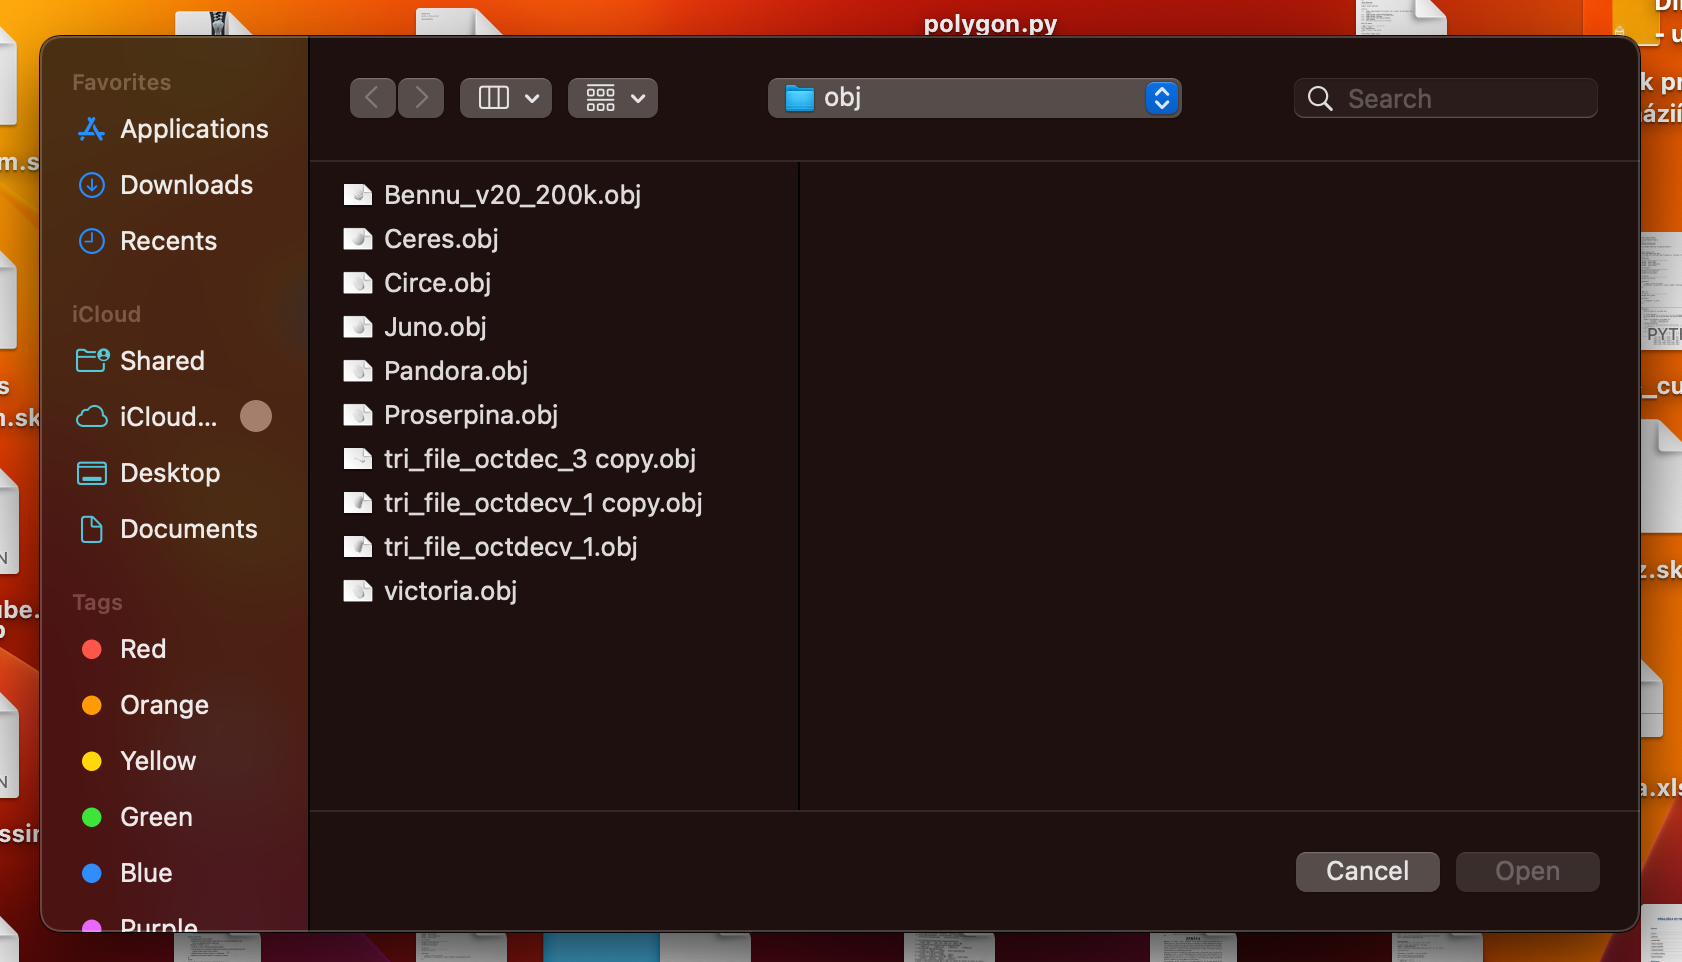
\includegraphics[width=10cm]{figs/tkinter.png}
\centering
\caption{Ukázka výběru souboru za pomoci knihovny Tkinter.}
\label{tkinter}
\end{figure}

Také se může stát, že uživatel nevybere žádný soubor. Program by pak měl skončit příslušným chybovým hlášením. Špatně vybraný i~nevybraný soubor řeší dvojce podmínek.

\lstinputlisting[language=Python,firstnumber=last]{python_scripts/3_8/ifs.py}

Nakonec funkce \verb|main()| zavolá konstruktor třídy \verb|Asteroid()|, s~informací o~terminálových argumentech a~cestě k~souboru, a~předá řízení smyčce knihovny VisPy.

\lstinputlisting[language=Python,firstnumber=last]{python_scripts/3_8/main_end.py}

\begin{figure}[h]
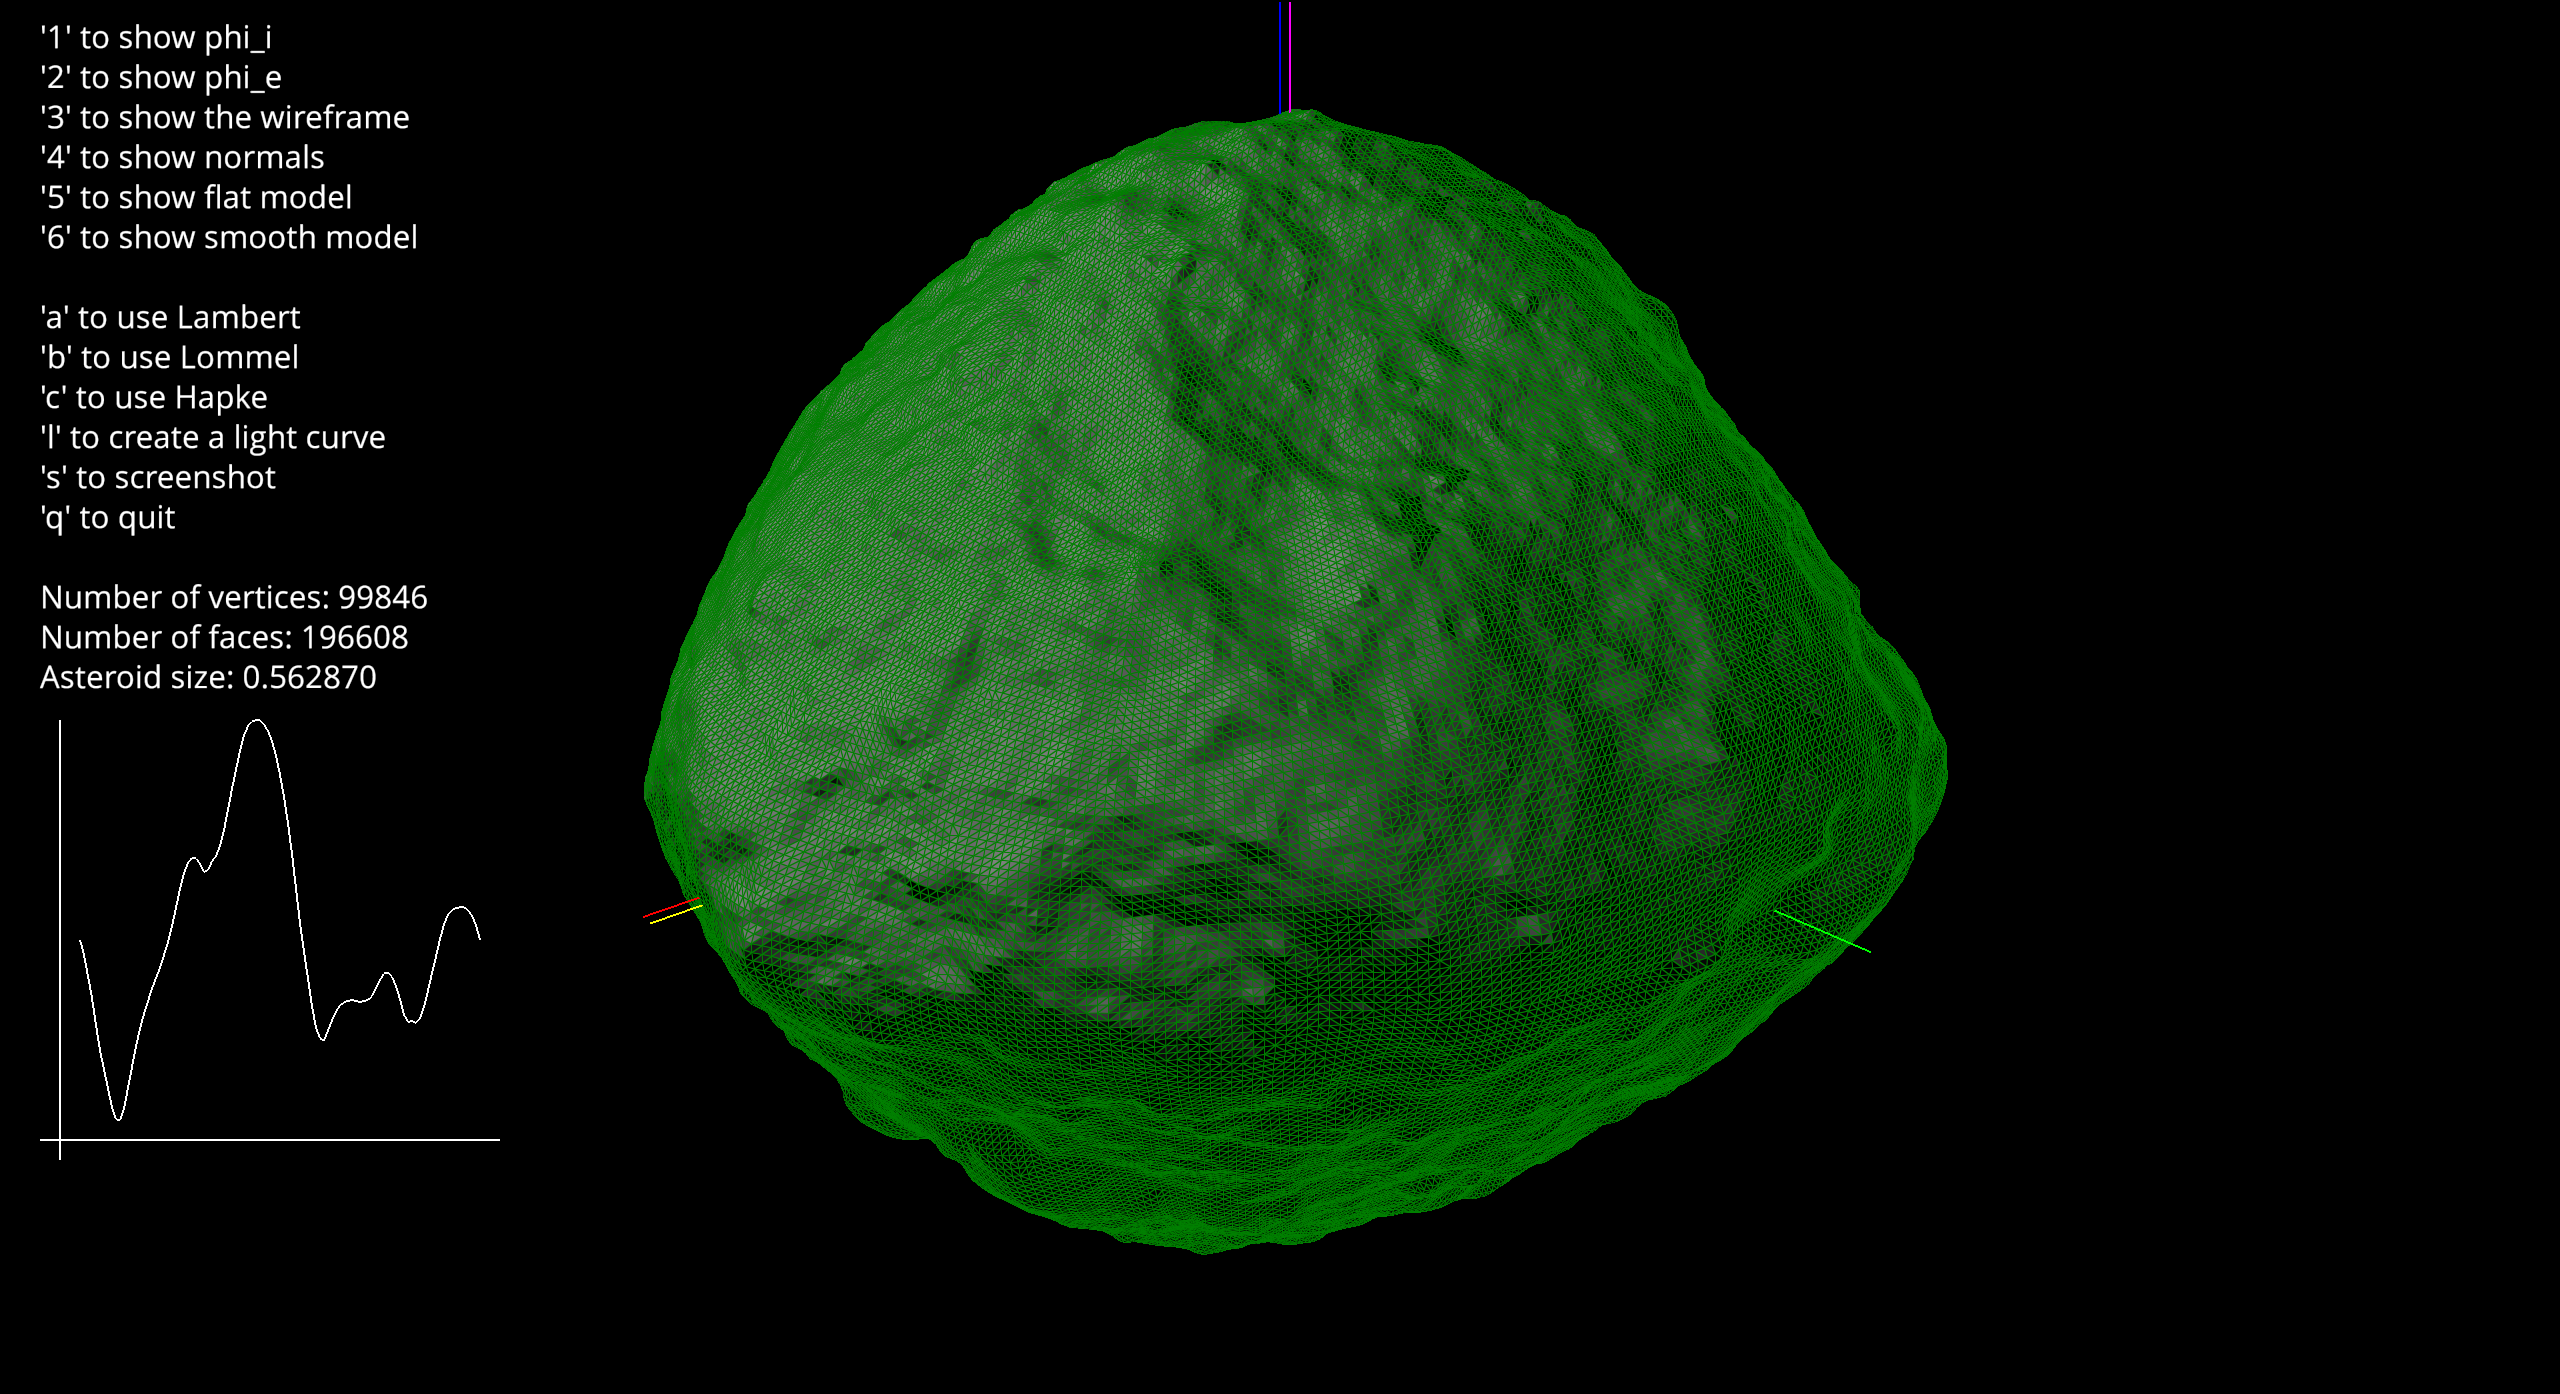
\includegraphics[width=12cm]{figs/Bennu.png}
\centering
\caption{Ukázka výstupu programu, model asteroidu (101955) Bennu s Hapkeho funkcí rozptylu,
vytvořený ze snímků pořízených sondou OSIRIS-REx, a jeho světelná křivka
\cite{Lauretta_2019Sci...366.3544L,Lauretta_2022Sci...377..285L}.
}
\label{bennu}
\end{figure}

%%%%%%%%%%%%%%%%%%%%%%%%%%%%%%%%%%%%%%%%%%%%%%%%%%%%%%%%%%%%%%%%%%%%%%

\newpage
\section{Produkt}

\subsection{Instalace}

Aby uživatel mohl aplikaci spustit, musí jeho počítač splňovat určité predispozice. Těmi jsou, mimo aplikace samotné, Python 3 \cite{python}, knihovna NumPy \cite{numpy} a nejnovější verze knihovny VisPy \cite{vispy}. 

\subsubsection{Instalace programovacího jazyka Python}

Nejnovější verze programovacího jazyka Python se nachází na domovské stránce, v~menu Downloads (\url{https://www.python.org/downloads/}). Python je multiplatformní interpretovaný jazyk, čili funguje na více operačních systémech. Instalací na MacOS provede uživatele stáhnutý soubor \verb|.pkg|. U ostatních systémů funguje instalace obdobně. Úspěšnost instalace pak můžeme ověřit příkazem \verb|python3 --version|, který by měl vrátit aktuální verzi nainstalovaného Pythonu. 

\subsubsection{Instalace knihovny NumPy}

Další velice důležitou predispozicí pro fungování programu je knihovna NumPy. Tu program používá pro komplexní matematické operace, využívající takzvaná {\em numpyovská pole\/}, která zrychlují operace, zejména for cykly. Knihovnu NumPy, stejně jako další zmíněné knihovny, lze instalovat přes terminálový nástroj zvaný \verb|pip|. Příkaz pro instalaci knihovny NumPy je uvedený níže.

\begin{lstlisting}
pip install numpy
\end{lstlisting}

Informace o tom, jak nainstalovat terminálový nástroj \verb|pip|, jsou dostupné na následující adrese, 
\url{https://pip.pypa.io/en/stable/installation/}.

\subsubsection{Instalace knihovny VisPy}

Knihovnu VisPy je lze nainstalovat příkazem uvedeným níže. Dokumentace knihovny VisPy a~detailnější popis její instalace je dostupný na stránce \cite{vispy}.

\begin{lstlisting}
pip install vispy
\end{lstlisting}

\subsubsection{Ostatní predispozice}

K dalším důležitým predispozicím patří knihovna Tk. Ta v~programu umožňuje výběr souboru pro vizualizaci. Aby se mohl program ke knihovně Tk dostat, potřebuje modul zvaný \verb|tkinter|. Ten je součástí pipu a lze jej nainstalovat příkazem níže. 

\begin{lstlisting}
pip install tk
\end{lstlisting}

Poslední knihovnou, která nesmí před spuštěním programu chybět, je Pyopelgl.

\begin{lstlisting}
pip install pyopengl
pip install pyopengltk
\end{lstlisting}

\subsubsection{Instalace samotné aplikace}

Nejaktuálnější verze zdrojového kódu je dostupná na stránce \url{https://github.com/scraptechguy/tvet}. Archiv \verb|.zip| stačí rozbalit do adresáře.

\subsection{Manuál}

Uživatel spustí program kliknutím na soubor \verb|Main.py|. Po spuštění, jak je vidět na obrázku~\ref{tkinter}, se aplikace zeptá na soubor \verb|.obj|, který má zobrazit. Při vybrání žádného, nebo jiného souboru, než je \verb|.obj|, program skončí s~příslušnou chybovou hláškou.

Poté, co uživatel vybere platný soubor, se otevře hlavní okno programu. V~něm uživatel uvidí zahlazený model asteroidu, nasvícený z~jednoho směru (obr.~\ref{bennu}). U tohoto zobrazení není počítané vzájemné stínění trojúhelníků. 

\begin{figure}[h]
\includegraphics[width=12cm]{figs/bennu_base.png}
\centering
\caption{Model asteroidu (101955) Bennu,
vytvořený ze snímků pořízených sondou OSIRIS-REx
\cite{Lauretta_2019Sci...366.3544L,Lauretta_2022Sci...377..285L}.
Zobrazení klávesou '6'.}
\label{bennu}
\end{figure}

Kromě základního modelu má uživatel přístup k pěti dalším, jejichž seznam s popisky je uveden níže. Přepínat modely uživatel může příslušnými klávesami (číslicemi '1' až '6').  

\begin{lstlisting}
'1' - model, ktery ukazuje phi_i
'2' - model, ktery ukazuje phi_e
'3' - model, ktery ukazuje pouze sit asteroidu
'4' - model, ktery ukazuje normaly trojuhelniku
'5' - hruby model asteroidu
'6' - hladky model asteroidu
\end{lstlisting}

\begin{figure}[h]
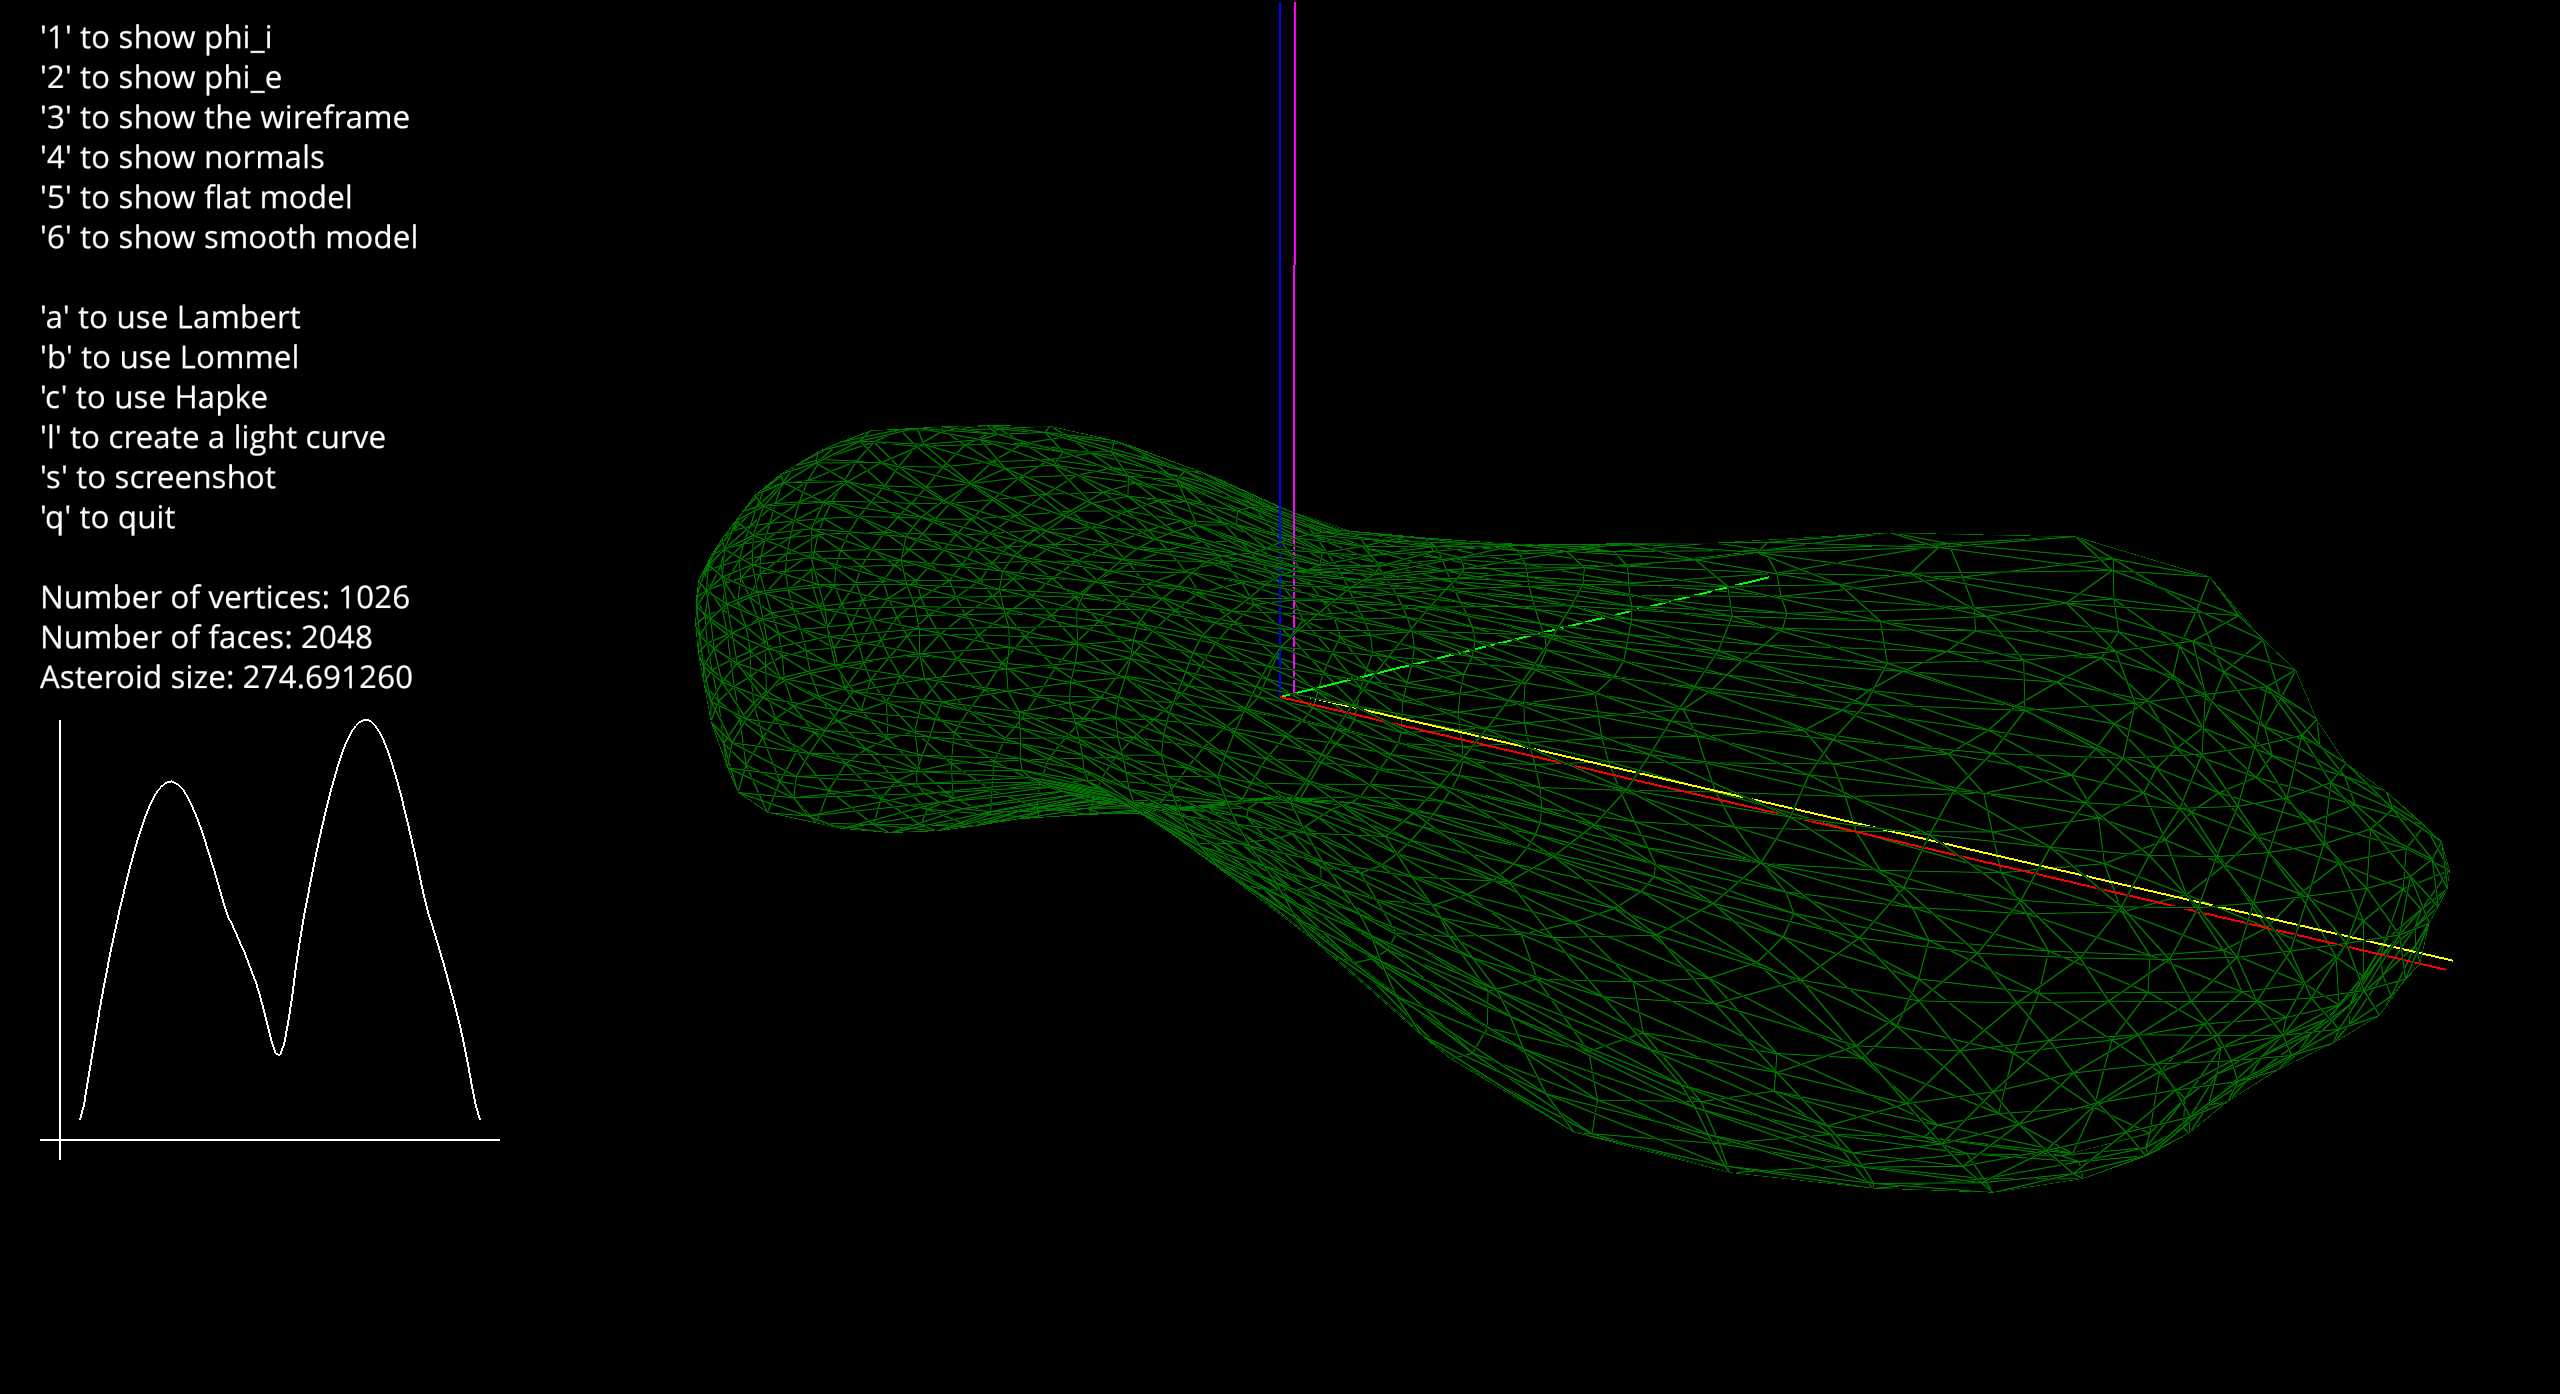
\includegraphics[width=12cm]{figs/Kleopatra.png}
\centering
\caption{Síť modelu asteroidu (216) Kleopatra \cite{Marchis_2021A&A...653A..57M,Broz_2021A&A...653A..56B}.
Zobrazení klávesou '3'.
}
\label{kleopatra}
\end{figure}

U druhého modelu se dá písmeny 'a', 'b' a 'c' volit funkce rozptylu. Další písmena pak umožňují dodatečné ovládání programu, jak je vidět v seznamu níže.

\begin{lstlisting}
'a' - pouzije Lambertuv rozptyl
'b' - pouzije Lommeluv-Seeligeruv rozptyl
'c' - pouzije Hapkeho rozptyl
'l' - vypocita svetelnou krivku
's' - udela snimek obrazovky
'q' - opusti aplikaci
\end{lstlisting}

Nad světelnou křivkou také program vypisuje počet vrcholů asteroidu, počet jeho stěn a velikost modelu. 

\begin{figure}[h]
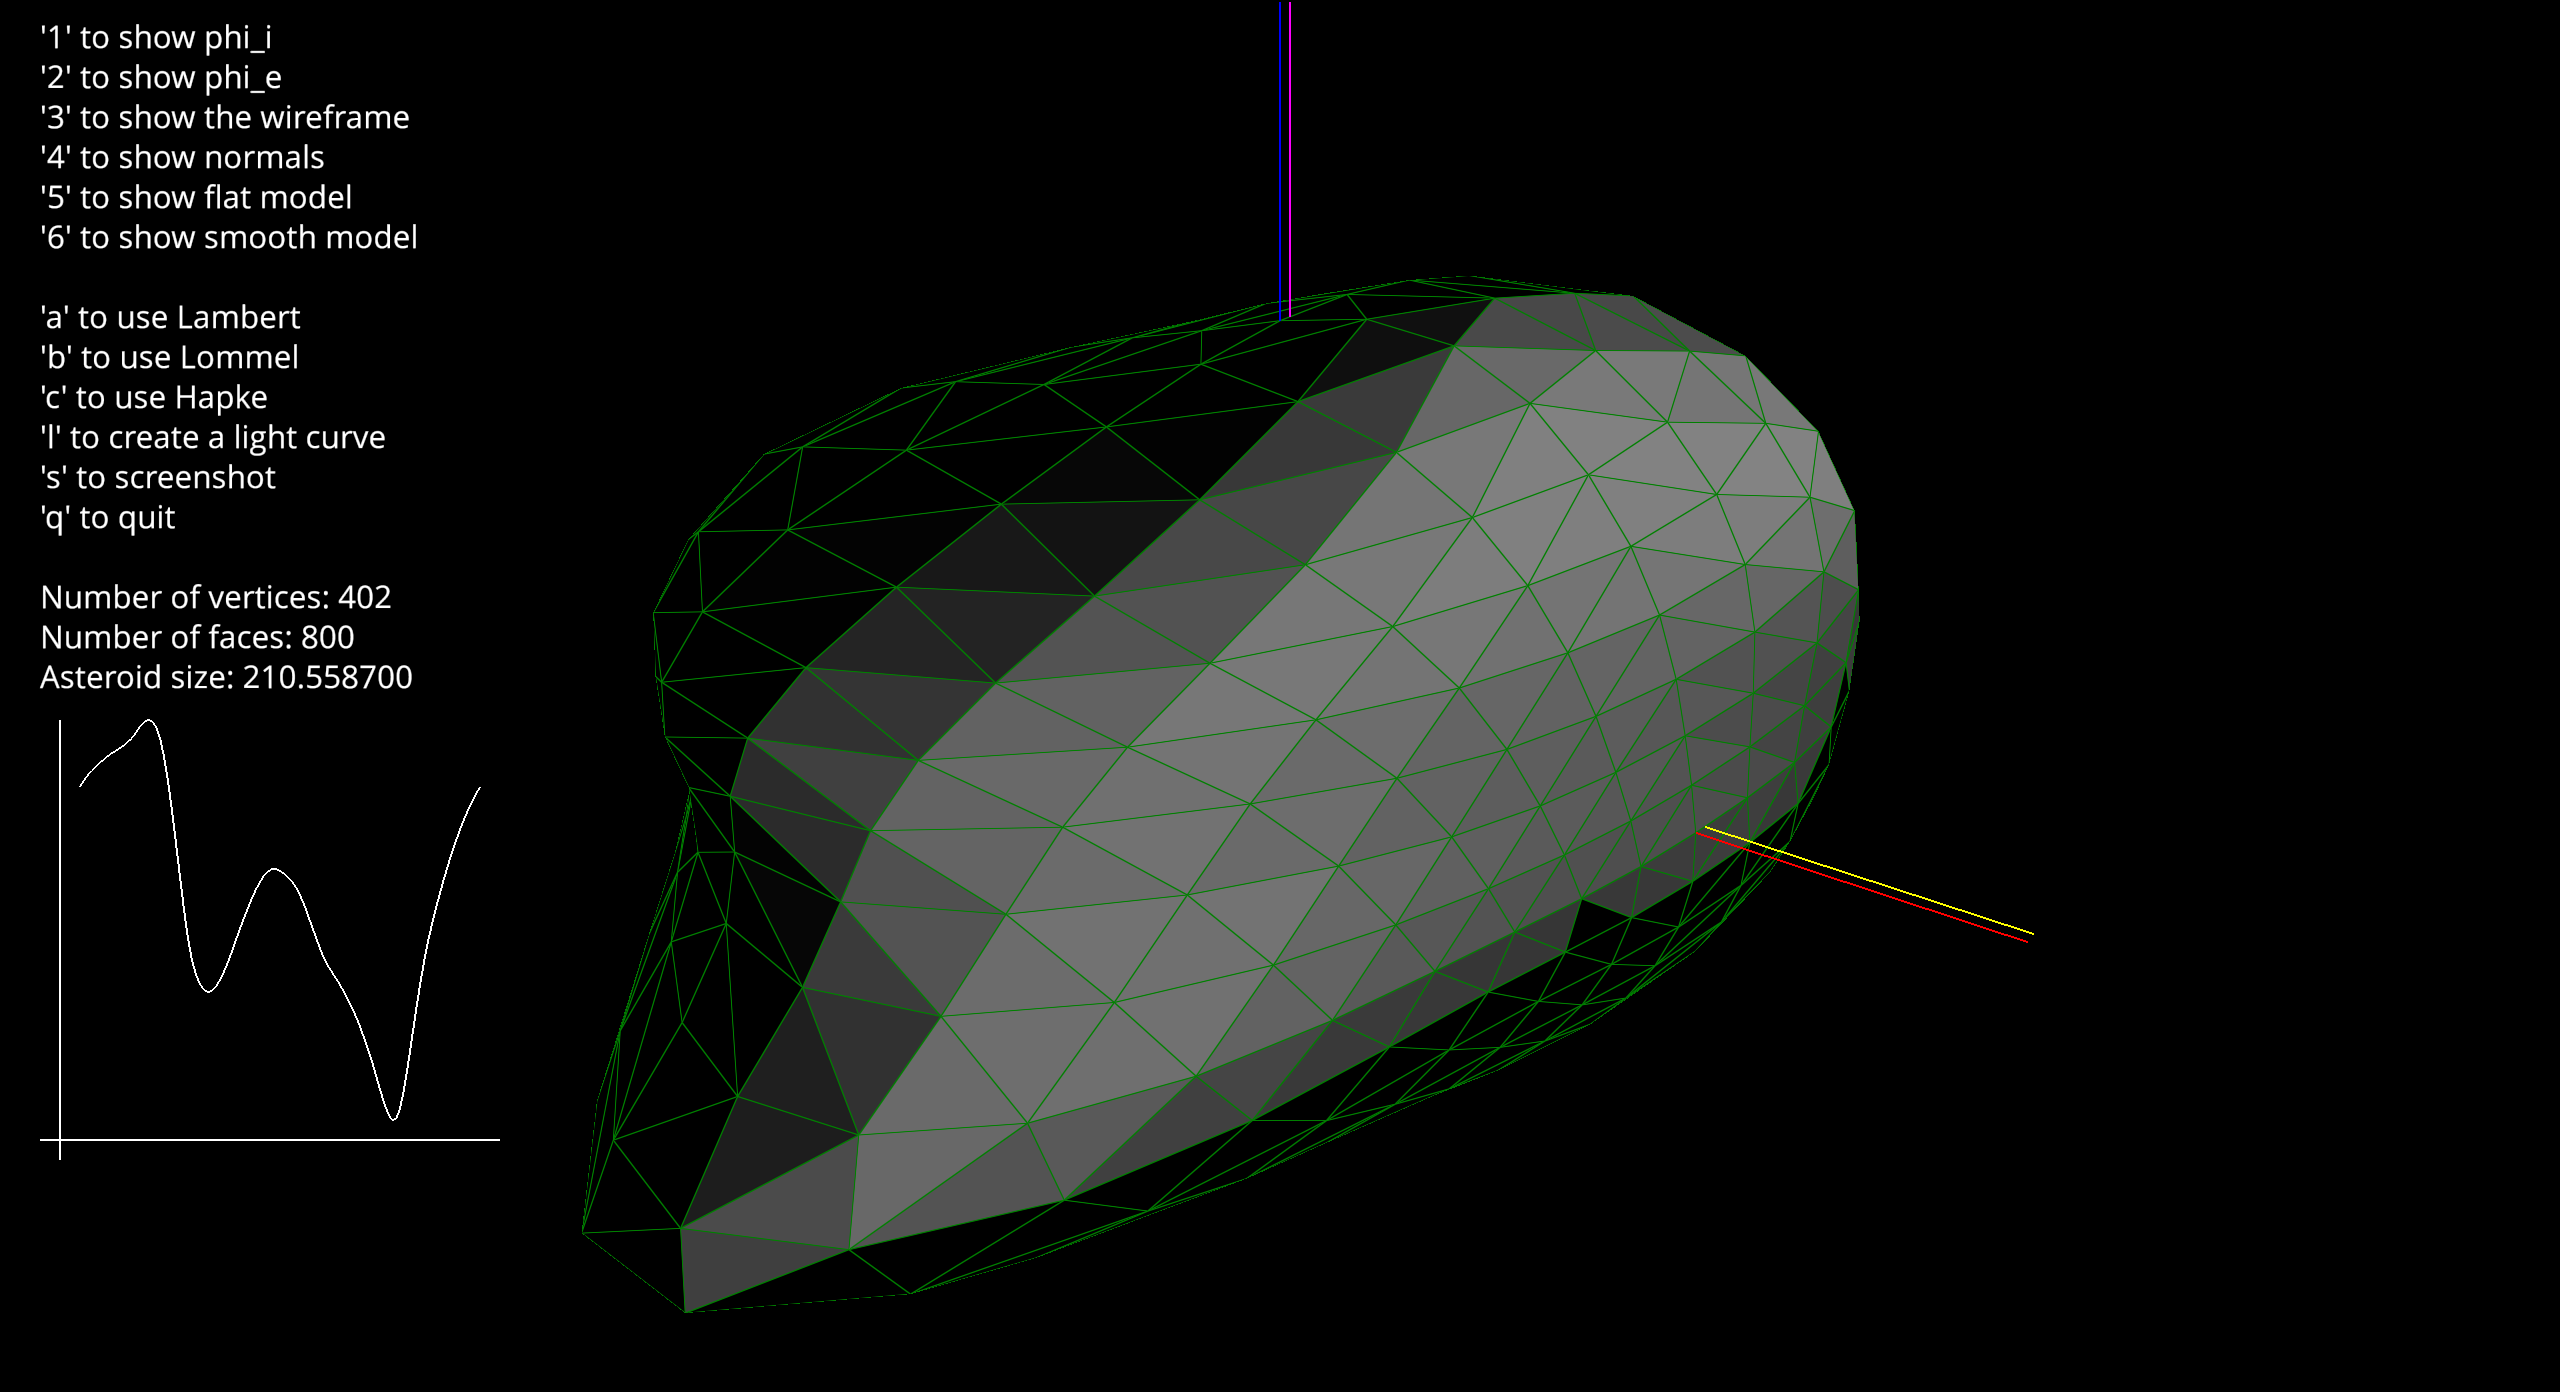
\includegraphics[width=12cm]{figs/Kalliope.png}
\centering
\caption{Model asteroidu (22) Kalliope s~Hapkeho funkcí rozptylu \cite{Ferrais_2022A&A...662A..71F,Broz_2023A&A...676A..60B}.
Zobrazení klávesami 'c'~+~'2'.
}
\label{kalliope}
\end{figure}


%%%%%%%%%%%%%%%%%%%%%%%%%%%%%%%%%%%%%%%%%%%%%%%%%%%%%%%%%%%%%%%%%%%%%%

\clearpage
\section*{Závěr}
\addcontentsline{toc}{section}{Závěr}

Cílem práce bylo vytvořit jednotný program pro vizualizaci asteroidů a jejich světelných křivek, který v komunitě astronomů chyběl. Cíl práce se podařil, program je funkční a dostupný veřejnosti. Program umí zpracovat soubor \verb|.obj| a zobrazit jej šesti různými způsoby a spočítat světelnou křivku. Povrch asteroidů umí popsat třemi různými funkcemi rozptylu, mezi kterými může uživatel přepínat klávesami. 

Celý program je psaný objektově, je rozdělený na třídu a její metody. Pro jiné vývojáře je tak velmi jednoduché program pochopit, dál na něm stavět a zlepšovat ho. Smysluplným rozšířením by bylo například napojení na databázi DAMIT \citep{Durech_2023A&A...675A..24D}, ve které se nachází tisíce modelů asteroidů, které by program mohl zobrazovat. Dále by bylo možné přidat načítání reálných efemerid z databáze JPL Horizons \citep{jpl_horizons}. 

%%%%%%%%%%%%%%%%%%%%%%%%%%%%%%%%%%%%%%%%%%%%%%%%%%%%%%%%%%%%%%%%%%%%%%

\newpage
\addcontentsline{toc}{section}{Zdroje}
\bibliographystyle{unsrt}
\bibliography{citace.bib}

\end{document}
